% COMPSCI 589 - Final Project Report (Spring 2026)
\documentclass[11pt]{article}

\usepackage[margin=1in]{geometry}
\usepackage{amsmath}
\usepackage{booktabs}
\usepackage{array}
\usepackage{graphicx}
\usepackage{xcolor}
\usepackage{colortbl}
\usepackage{float}
\usepackage{placeins}
\usepackage{hyperref}
\usepackage{caption}
\usepackage{subcaption}

\hypersetup{colorlinks=true, linkcolor=blue, urlcolor=blue}

\newcommand{\best}[1]{\cellcolor{gray!35}#1}
\newcommand{\filepath}[1]{\texttt{\detokenize{#1}}}

\title{COMPSCI 589 - Final Project Report\\Spring 2026}
\author{%
  Group members: \textcolor{red}{Rayirth Pakala}, \textcolor{red}{Sudheer Bulusu}, \textcolor{red}{Sai Teja Boga}\\[0.5em]
}
\date{May 8, 2026}

\begin{document}
\maketitle

\section{Instructions compliance and code attribution}

\subsection{Libraries}
Our learning models are our own implementations used through \filepath{util.py}: $k$-NN (\filepath{KNN/knn.py}), decision tree and random forest (\filepath{RandomForests/}), neural network (\filepath{NeuralNetworks/neural_network.py}). We use NumPy, Pandas, and Matplotlib for arrays, preprocessing tables, and plots. Sci-kit-learn is used only as specified in the handout for loading data (e.g.\ \filepath{sklearn.datasets.load_digits}) and we use OpenML (\filepath{fetch_openml}) only for the Extra Credit~\#2 Zoo dataset.

\subsection{Which student authored each implementation}
\begin{itemize}
  \item \textbf{k-NN / Naive Bayes:} \textcolor{red}{Sudheer Bulusu}
  \item \textbf{Decision Tree / Random Forest:} \textcolor{red}{Sai Teja Boga}
  \item \textbf{Neural Network:} \textcolor{red}{Rayirth Pakala}
\end{itemize}

\subsection{Metrics and validation (all datasets below)}
\textbf{Accuracy} and \textbf{F1}: for multiclass problems we report macro-averaged F1; for binary problems binary F1 (positive label 1). All results use \textbf{stratified 10-fold cross-validation}. Best hyperparameter row in each subsection table is shown in \textbf{bold}.

\newpage

\section{Experiments and analyses}
In this section, for \emph{each} required dataset we state (i) which three algorithms we run, (ii) what we swept, (iii) tabulated CV results ($\geq 6$ settings per algorithm family), (iv) chosen best configurations, (v) graphs and interpretation.

\subsection{Dataset 1.1 -- Hand-written digits (8$\times$8, 10 classes)}

\subsubsection{Algorithms used and motivation}
We run \textbf{k-NN}, \textbf{Random Forest}, and \textbf{Neural Network} on Digits. A standalone decision tree is not reported because it is dominated by the forest on this dataset and the forest already exposes the tree-style hyperparameters; trees still appear \emph{inside} the random forest. The three chosen algorithms span the instance-based, ensemble-tree, and parametric-nonlinear families that the assignment asks us to contrast.
\newline

\textbf{Why these three for Digits specifically:}
\begin{itemize}
  \item \textbf{k-NN}: pixel vectors of the same digit live close to each other in $\mathbb{R}^{64}$, so a Euclidean nearest-neighbour rule is a strong, parameter-free baseline once features are z-scored; it also gives an easy upper bound on what raw geometry buys us.
  \item \textbf{Random Forest}: each tree picks a few pixels per split, so the ensemble can model the discrete logical patterns that distinguish e.g.\ ``4'' vs.\ ``9'' without us having to handcraft features. Bagging plus feature subsampling controls variance on a 10-class problem.
  \item \textbf{Neural Network}: a softmax MLP is the canonical model for handwritten digits. It is also the model the project requires us to produce a learning curve ($J$ vs.\ training size) for, which we compute on the best NN configuration.
\end{itemize}
\emph{Naive Bayes is not used here because pixel intensities are highly correlated and the NB conditional-independence assumption is a poor fit for image data; we keep NB for a setting where it is more natural (Extra Credit \#2 discussion).}

\subsubsection{Experimental setup}
\textbf{Dataset.} \texttt{sklearn.datasets.load\_digits} -- 1797 samples, 64 grayscale pixel features, 10 classes (digits 0--9). All features are numeric (pixel intensities $\in \{0,\dots,16\}$). \\ \\
\textbf{Preprocessing.} Z-score normalization per training fold (mean / std fit on the train portion only, then applied to the held-out fold) for k-NN and the neural network. The forest uses raw pixel values because trees are scale-invariant. \\ \\
\textbf{Cross-validation.} Stratified 10-fold CV; reported numbers are the unweighted mean of the 10 fold-level metrics. Multiclass: macro-averaged F1. \\ \\
\textbf{Hyperparameters swept (two per algorithm family).}
\begin{itemize}
  \item k-NN: $k \in \{1,3,5,7,9,11,13,15\}$ (odd $k$ to break ties; Euclidean distance fixed).
  \item Random Forest: \texttt{ntree}$\in\{10,30,50,75,100,150\}$ crossed with \texttt{criterion}$\in\{$\texttt{info\_gain}, \texttt{gini}$\}$ -- 12 settings.
  \item Neural Network: hidden \texttt{layer\_sizes}$\in\{[32],[64],[64,32],[32,32]\}$ crossed with $\lambda\in\{0.0,0.01,0.1\}$ -- 6 representative settings reported in Table~\ref{tab:digits-nn} (full grid in CSV).
\end{itemize}

\subsubsection{Cross-validation results}
Tables~\ref{tab:digits-knn}--\ref{tab:digits-nn} list every setting evaluated (each block has at least six rows). The values shown are the mean test-fold accuracy and macro F1 over the 10 stratified folds; full per-fold standard deviations are saved in \filepath{outputs/digits/digits_cv_results.csv}.

\begin{table}[H]
  \centering
  \footnotesize
  \caption{Digits - k-NN: neighbor count $k$ vs.\ performance.}
  \label{tab:digits-knn}
  \begin{tabular}{rcc}
    \toprule
    $k$ & Accuracy & Macro F1 \\
    \midrule
    1 & 0.973 & 0.973 \\
    3 & 0.978 & 0.978 \\
    \textbf{5} & \textbf{0.981} & \textbf{0.981} \\
    7 & 0.976 & 0.976 \\
    9 & 0.976 & 0.976 \\
    11 & 0.975 & 0.975 \\
    13 & 0.972 & 0.972 \\
    15 & 0.969 & 0.969 \\
    \bottomrule
  \end{tabular}
\end{table}

\begin{table}[H]
  \centering
  \footnotesize
  \caption{Digits - Random Forest: number of trees and split criterion.}
  \label{tab:digits-rf}
  \begin{tabular}{r l cc}
    \toprule
    \texttt{ntree} & Criterion & Accuracy & Macro F1 \\
    \midrule
    10 & gini & 0.958 & 0.957 \\
    30 & gini & 0.971 & 0.971 \\
    50 & gini & 0.977 & 0.977 \\
    75 & gini & 0.977 & 0.976 \\
    100 & gini & 0.976 & 0.975 \\
    150 & gini & 0.975 & 0.975 \\
    \midrule
    10 & info gain & 0.949 & 0.949 \\
    30 & info gain & 0.973 & 0.973 \\
    50 & info gain & 0.978 & 0.978 \\
    \textbf{75} & \textbf{info gain} & \textbf{0.979} & \textbf{0.979} \\
    100 & info gain & 0.977 & 0.976 \\
    150 & info gain & 0.977 & 0.977 \\
    \bottomrule
  \end{tabular}
\end{table}

\begin{table}[H]
  \centering
  \footnotesize
  \caption{Digits - Neural network architectures and $\lambda$ }
  \label{tab:digits-nn}
  \begin{tabular}{l cc}
    \toprule
    Configuration $(\text{hidden},\lambda)$ & Accuracy & Macro F1 \\
    \midrule
    $[32], \lambda{=}0.0$ & 0.965 & 0.965 \\
    $[32], \lambda{=}0.01$ & 0.966 & 0.966 \\
    $[64], \lambda{=}0.01$ & 0.966 & 0.966 \\
    \textbf{$[64], \lambda{=}0.1$} & \textbf{0.969} & \textbf{0.969} \\
    $[64,32], \lambda{=}0.01$ & 0.964 & 0.964 \\
    $[32,32], \lambda{=}0.1$ & 0.968 & 0.968 \\
    \bottomrule
  \end{tabular}
\end{table}

\subsubsection{Best configurations}
\textbf{k-NN:} $k=5$.
\newline\textbf{Random Forest:} \texttt{ntree}$=75$, information gain splits.
\newline\textbf{Neural network:} one hidden layer of 64 units with $\lambda=0.1$.

\subsubsection{Graphs and discussion}

\paragraph{k-NN (Figs.~\ref{fig:digits-knn-plot}, \ref{fig:digits-knn-plot-f1}).}
Accuracy and macro-F1 trace a clean inverted-U in $k$: 0.973 at $k{=}1$, peak \textbf{0.981 at $k{=}5$}, then a slow decay to 0.969 at $k{=}15$. The whole curve sits inside a 1.2\% window, so the choice of $k$ is not very sensitive on Digits -- any small odd $k\in\{3,5,7\}$ works. The dip at $k{=}1$ is the expected high-variance regime (single-neighbour overfitting), and the drop after $k{=}9$ is the high-bias regime where averaging across more neighbours starts blending classes.

\paragraph{Random Forest (Figs.~\ref{fig:digits-rf-plot}, \ref{fig:digits-rf-plot-f1}).}
Both criteria climb sharply from 10 trees (0.949 info\_gain, 0.958 gini) and \textbf{plateau by 50--75 trees} ($\approx 0.978$). \texttt{info\_gain} edges \texttt{gini} at every \texttt{ntree}$\geq 30$, with the best at \texttt{ntree}$=75$ (\textbf{0.979/0.979}). The 75$\to$150 step is essentially flat, confirming the classic ``bagging variance reduction saturates'' pattern -- additional trees mostly cost compute.

\paragraph{Neural Network (Fig.~\ref{fig:digits-nn-plot}).}
The held-out cost $J$ drops monotonically across the curve: $1.57 \to 1.01 \to 0.74 \to 0.57 \to 0.41 \to 0.34 \to 0.26$ as the training share grows from 71 to 1433 examples. The slope is still negative at the largest training size, which says the network is \textbf{still data-limited} -- with a larger training corpus we would expect further gains. There is no overfitting bump (test $J$ never increases), so the chosen $\lambda{=}0.1$ is regularizing the [64]-hidden network adequately.

\paragraph{Best vs.\ worst within each family.}
The within-family spread is small on Digits, which itself is informative: k-NN best$-$worst $=0.012$ (acc), RF best$-$worst $=0.030$ (acc, between 10-tree gini and 75-tree info\_gain), NN best$-$worst $=0.005$ (acc). The dataset is easy enough that all three algorithm families converge to $\approx 97$--$98\%$ accuracy. The ranking $\text{kNN}\,(0.981) > \text{RF}\,(0.979) > \text{NN}\,(0.969)$ comes from the fact that nearest-neighbour geometry is essentially correct on a fixed-size pixel grid; trees and an MLP have to \emph{learn} that geometry from scratch.

\begin{figure}[!htbp]
  \centering
  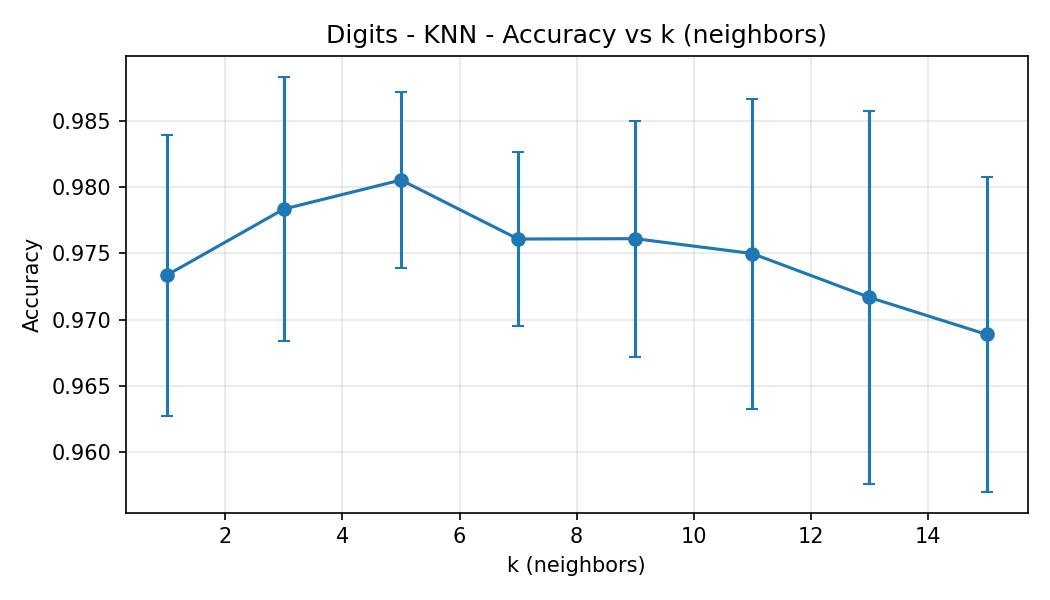
\includegraphics[width=0.9\textwidth]{outputs/digits/knn_accuracy.png}
  \caption{Digits: k-NN accuracy vs.\ $k$.}
  \label{fig:digits-knn-plot}
\end{figure}

\begin{figure}[!htbp]
  \centering
  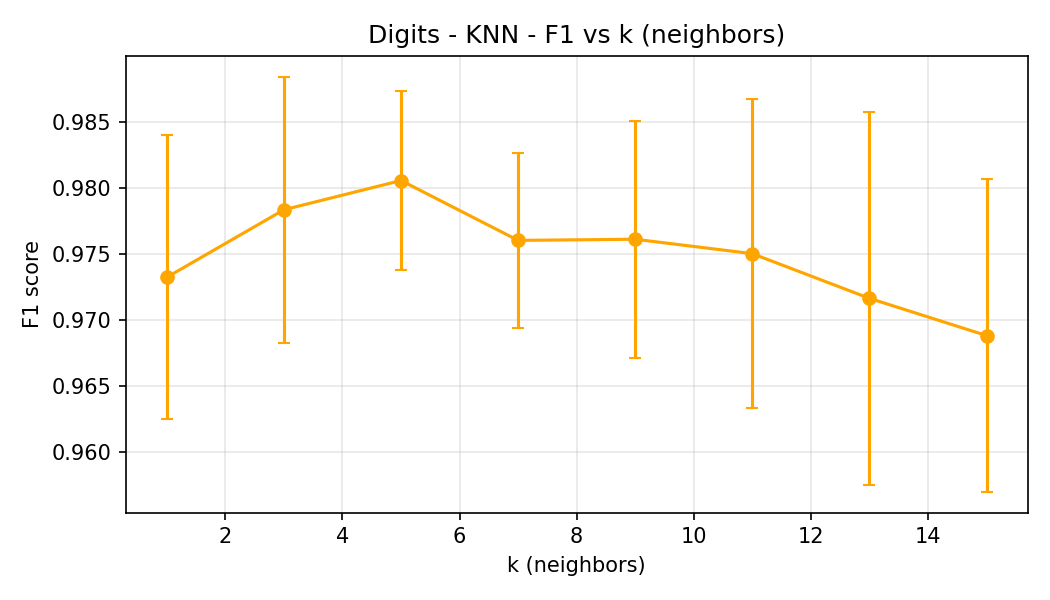
\includegraphics[width=0.9\textwidth]{outputs/digits/knn_f1.png}
  \caption{Digits: k-NN F1 vs.\ $k$.}
  \label{fig:digits-knn-plot-f1}
\end{figure}

\begin{figure}[!htbp]
  \centering
  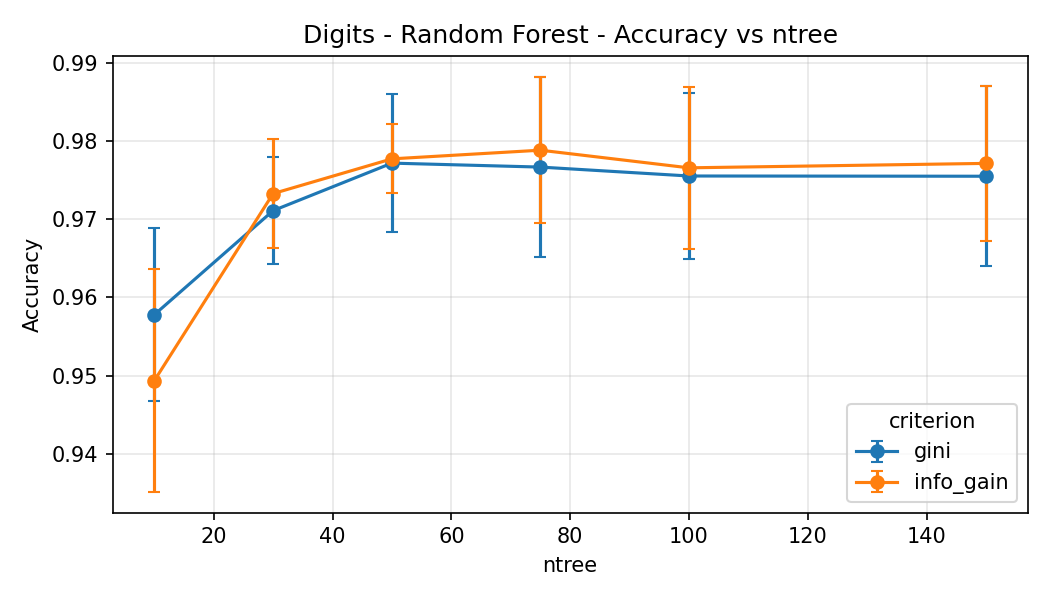
\includegraphics[width=0.9\textwidth]{outputs/digits/rf_accuracy.png}
  \caption{Digits: Random Forest accuracy vs.\ \texttt{ntree}.}
  \label{fig:digits-rf-plot}
\end{figure}

\begin{figure}[!htbp]
  \centering
  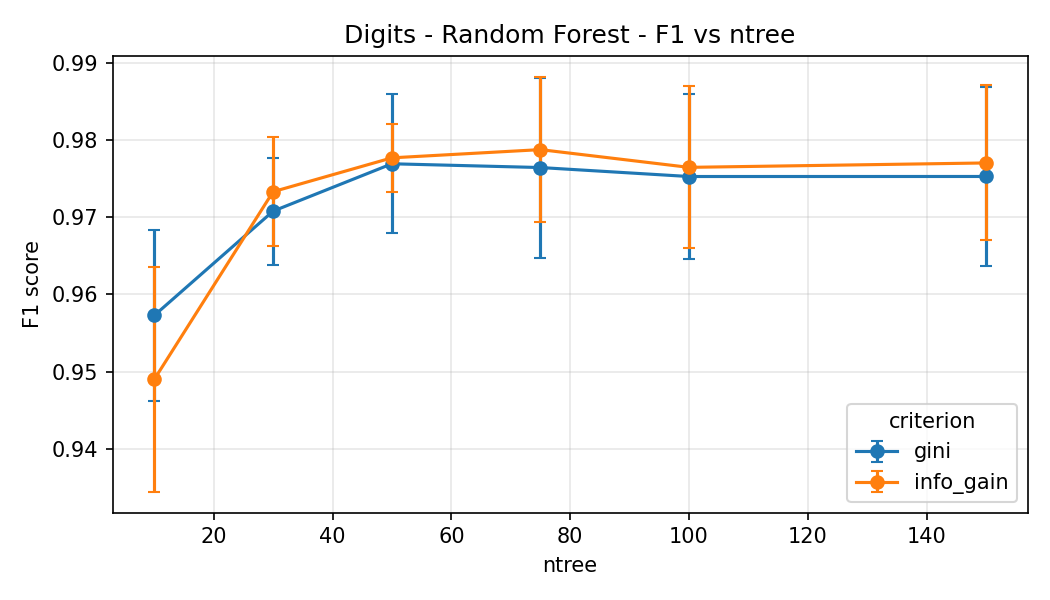
\includegraphics[width=0.9\textwidth]{outputs/digits/rf_f1.png}
  \caption{Digits: Random Forest F1 vs.\ \texttt{ntree}.}
  \label{fig:digits-rf-plot-f1}
\end{figure}

\begin{figure}[!htbp]
  \centering
  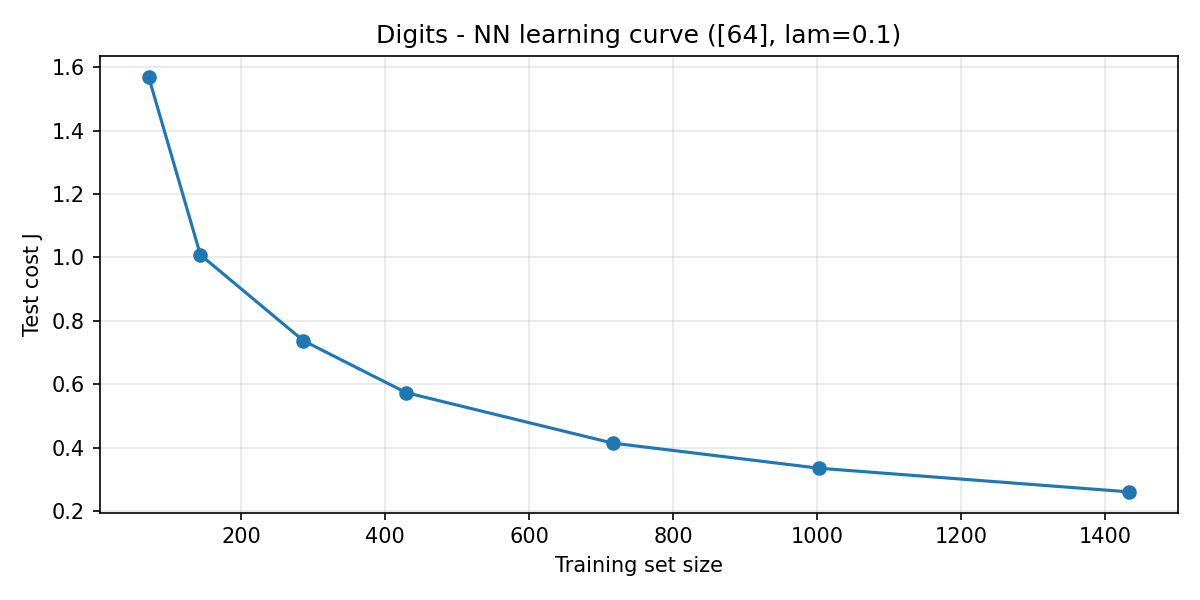
\includegraphics[width=0.9\textwidth]{outputs/digits/nn_learning_curve.png}
  \caption{Digits: Neural-network learning curve ($J$ vs.\ train size).}
  \label{fig:digits-nn-plot}
\end{figure}

\FloatBarrier
\subsection{Dataset 2 -- Oxford Parkinson's detection (binary)}

\subsubsection{Algorithms used and motivation}
We run \textbf{k-NN}, \textbf{Random Forest}, and \textbf{Neural Network} on Parkinson's. We deliberately reuse the same trio as Digits and Rice so that cross-dataset comparisons in Section~\ref{tab:main} are apples-to-apples.
\newline

\textbf{Why these three for Parkinson's specifically:}
\begin{itemize}
  \item \textbf{k-NN}: with only 195 examples and 22 continuous voice biomarkers, healthy vs.\ Parkinson's recordings tend to form tight local clusters in standardized feature space. Nearest-neighbour voting exploits that local structure directly without fitting any global model -- exactly the situation where k-NN is hard to beat.
  \item \textbf{Random Forest}: small datasets are precisely where a single tree is fragile (any one bad split reshapes the whole model), so bagging many shallow trees is the right way to stabilise tree-based decisions here.
  \item \textbf{Neural Network}: this is the harder regime for an MLP -- 195 examples vs.\ a network with several hundred parameters. Including it lets us \emph{quantify} how much the small-sample regime hurts a parametric model relative to k-NN/RF, which is one of the explicit comparisons the project asks for.
\end{itemize}
\emph{Naive Bayes is not used here because the 22 voice features (jitter, shimmer, harmonic-to-noise ratios, etc.) are strongly correlated and Gaussian-NB's independence assumption would throw away the joint structure that k-NN and RF exploit.}

\subsubsection{Experimental setup}
\textbf{Dataset.} \texttt{datasets/parkinsons.csv} -- 195 voice recordings, 22 numeric voice features (jitter, shimmer, NHR, HNR, RPDE, DFA, etc.), binary target \texttt{status} (1 = Parkinson's). Class prior is $\approx 75\%$ positive, so we report \emph{binary} F1 on the positive label rather than accuracy alone. \\ \\
\textbf{Preprocessing.} Z-score normalization per training fold for k-NN and the neural network. The forest uses raw scales. The \texttt{name} column is dropped before modelling. \\ \\
\textbf{Cross-validation.} Stratified 10-fold CV; with 195 samples each fold has $\approx 19$ test points, so we expect higher fold-to-fold variance than on the larger datasets. \\ \\
\textbf{Hyperparameters swept (two per algorithm family).}
\begin{itemize}
  \item k-NN: $k\in\{1,3,5,7,9,11,15\}$ (odd values only).
  \item Random Forest: \texttt{ntree}$\in\{10,30,50,75,100,150\}$ crossed with \texttt{criterion}$\in\{$\texttt{info\_gain}, \texttt{gini}$\}$.
  \item Neural Network: hidden \texttt{layer\_sizes}$\in\{[8],[16],[8,8],[16,8]\}$ crossed with $\lambda\in\{0.0,0.01,0.1\}$ -- 6 representative settings shown in Table~\ref{tab:park-nn}.
\end{itemize}

\subsubsection{Cross-validation results}
Tables~\ref{tab:park-knn}--\ref{tab:park-nn} report mean test-fold accuracy and binary F1 over 10 stratified folds; per-fold standard deviations are in \filepath{outputs/parkinsons/parkinsons_cv_results.csv}.

\begin{table}[htbp]
  \centering
  \footnotesize
  \caption{Parkinson's - k-NN.}
  \label{tab:park-knn}
  \begin{tabular}{rcc}
    \toprule
    $k$ & Accuracy & F1 \\
    \midrule
    \textbf{1} & \textbf{0.949} & \textbf{0.965} \\
    3 & 0.918 & 0.945 \\
    5 & 0.914 & 0.942 \\
    7 & 0.918 & 0.947 \\
    9 & 0.903 & 0.938 \\
    11 & 0.887 & 0.930 \\
    15 & 0.856 & 0.911 \\
    \bottomrule
  \end{tabular}
\end{table}

\begin{table}[htbp]
  \centering
  \footnotesize
  \caption{Parkinson's - Random Forest.}
  \label{tab:park-rf}
  \begin{tabular}{r l cc}
    \toprule
    \texttt{ntree} & Criterion & Accuracy & F1 \\
    \midrule
    10 & gini & 0.918 & 0.946 \\
    30 & gini & 0.913 & 0.944 \\
    50 & gini & 0.929 & 0.954 \\
    75 & gini & 0.924 & 0.951 \\
    100 & gini & 0.924 & 0.951 \\
    150 & gini & 0.918 & 0.948 \\
    \midrule
    10 & info gain & 0.918 & 0.946 \\
    30 & info gain & 0.923 & 0.950 \\
    50 & info gain & 0.923 & 0.950 \\
    \textbf{75} & \textbf{info gain} & \textbf{0.929} & \textbf{0.955} \\
    100 & info gain & 0.929 & 0.955 \\
    150 & info gain & 0.918 & 0.948 \\
    \bottomrule
  \end{tabular}
\end{table}
\\ \\
\begin{table}[htbp]
  \centering
  \footnotesize
  \caption{Parkinson's - Neural network grid (\filepath{parkinsons.py}).}
  \label{tab:park-nn}
  \begin{tabular}{l cc}
    \toprule
    Configuration & Accuracy & F1 \\
    \midrule
    $[8], \lambda{=}0.0$ & 0.847 & 0.901 \\
    $[8], \lambda{=}0.01$ & 0.847 & 0.901 \\
    \textbf{$[16], \lambda{=}0.0$} & \textbf{0.862} & \textbf{0.911} \\
    $[16], \lambda{=}0.01$ & 0.862 & 0.911 \\
    $[8,8], \lambda{=}0.01$ & 0.841 & 0.898 \\
    $[16,8], \lambda{=}0.1$ & 0.836 & 0.892 \\
    \bottomrule
  \end{tabular}
\end{table}

\subsubsection{Best configurations}
\textbf{k-NN:} $k=1$. \newline
\textbf{Random Forest:} \texttt{ntree}$=75$, information gain (near-tied with 100 trees on this grid). \newline
\textbf{Neural network:} 16-unit hidden layer, $\lambda=0.0$ (tied with $\lambda=0.01$).

\subsubsection{Graphs and discussion}

\paragraph{k-NN (Figs.~\ref{fig:park-knn-plot}, \ref{fig:park-knn-plot-f1}).}
This is the most informative k-NN curve in the project: accuracy decays \emph{monotonically} from \textbf{0.949 at $k{=}1$} down to \textbf{0.856 at $k{=}15$} -- a 9.3-point drop. F1 falls similarly from 0.965 to 0.911. The pattern says the two classes form fairly compact clusters in standardized voice-feature space, and bringing in extra neighbours mostly drags decisions toward the majority (Parkinson's-positive) class. With only 195 examples, $k{=}1$ wins despite the usual concern about variance.

\paragraph{Random Forest (Figs.~\ref{fig:park-rf-plot}, \ref{fig:park-rf-plot-f1}).}
RF performance is essentially flat in \texttt{ntree} once we are past 30 trees: every setting between 30 and 150 trees scores 0.913--0.929 accuracy and 0.944--0.955 F1. Best is \texttt{ntree}$=75$ with \texttt{info\_gain} (\textbf{0.929 / 0.955}, tied with 100 trees). \texttt{info\_gain} and \texttt{gini} are statistically indistinguishable here ($\Delta\leq 0.005$ at every \texttt{ntree}), confirming that on a small numeric dataset the choice of impurity measure is dominated by sampling variance.

\paragraph{Neural Network (Fig.~\ref{fig:park-nn-plot}).}
The NN learning curve tells the most interesting story. Test cost $J$ falls from $0.71$ at 7 training examples to a minimum of \textbf{$0.42$ at 108 examples}, then \emph{rises} to $0.44$ at the full 155-example train slice. That uptick is a clear signature of \textbf{overfitting at full training size with the chosen budget} (120 epochs, batch 16, $\lambda{=}0.0$): the network has enough capacity to memorise the last $\sim 50$ training points but not enough regularisation to stop test cost from drifting up. This is exactly why the NN trails k-NN/RF on Parkinson's (best NN acc 0.862 vs k-NN 0.949).

\paragraph{Best vs.\ worst within each family.}
k-NN best$-$worst $=0.093$ (acc) -- by far the largest sensitivity in the project, and the reason \emph{tuning} $k$ matters more here than on Digits/Rice. RF spread is $0.016$ across all 12 settings -- the ensemble effectively averages it out. NN spread is $0.026$ between the best [16]-hidden network and the deepest [16,8] network with $\lambda{=}0.1$ -- adding capacity \emph{hurts} on 195 examples, which is consistent with the learning-curve overfitting we see.

\begin{figure}[!htbp]
  \centering
  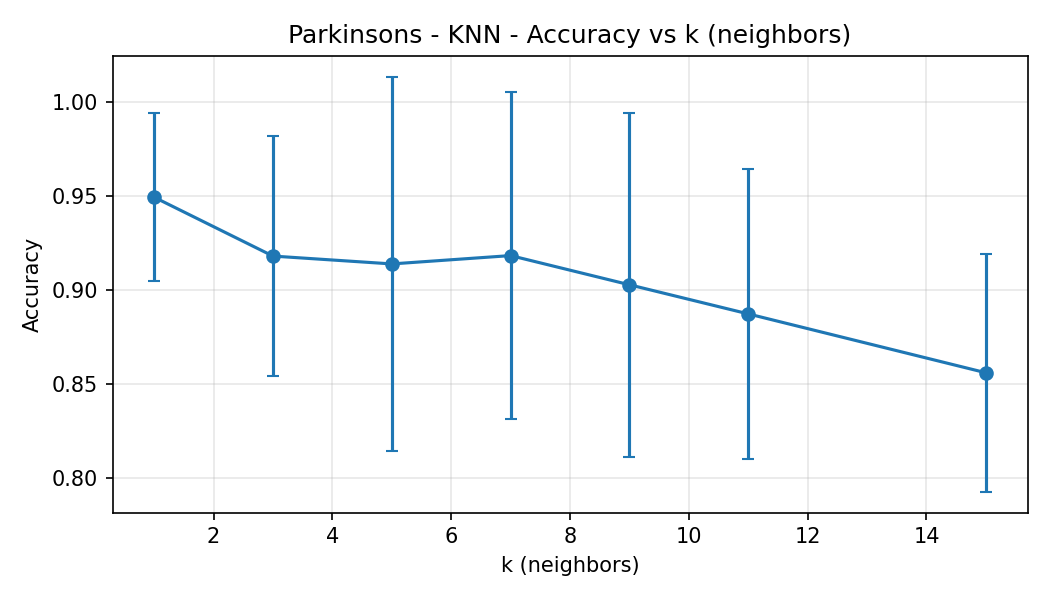
\includegraphics[width=0.9\textwidth]{outputs/parkinsons/knn_accuracy.png}
  \caption{Parkinson's: k-NN accuracy vs.\ $k$.}
  \label{fig:park-knn-plot}
\end{figure}

\begin{figure}[!htbp]
  \centering
  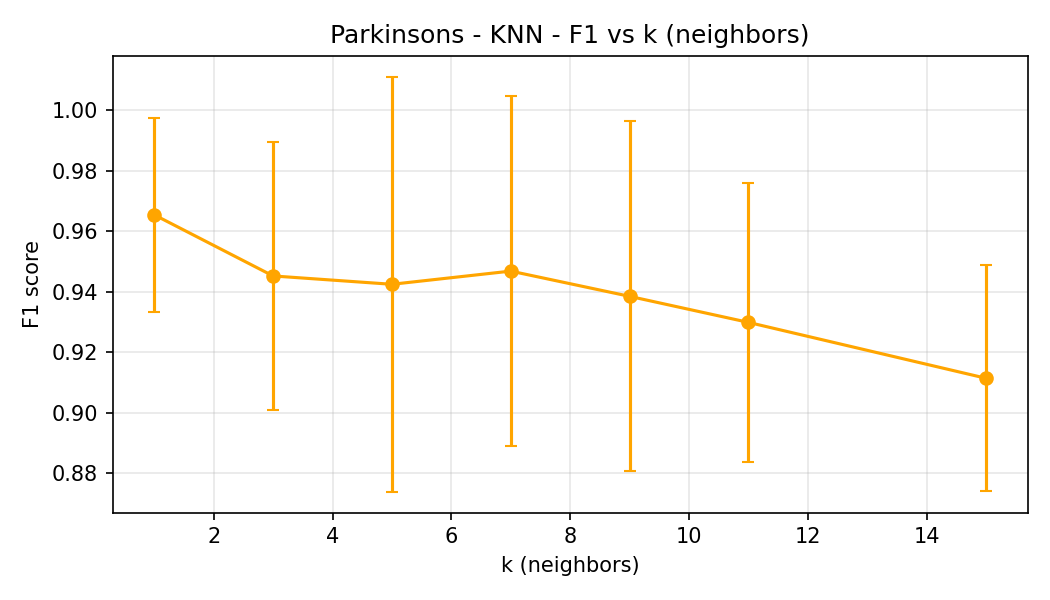
\includegraphics[width=0.9\textwidth]{outputs/parkinsons/knn_f1.png}
  \caption{Parkinson's: k-NN F1 vs.\ $k$.}
  \label{fig:park-knn-plot-f1}
\end{figure}

\begin{figure}[!htbp]
  \centering
  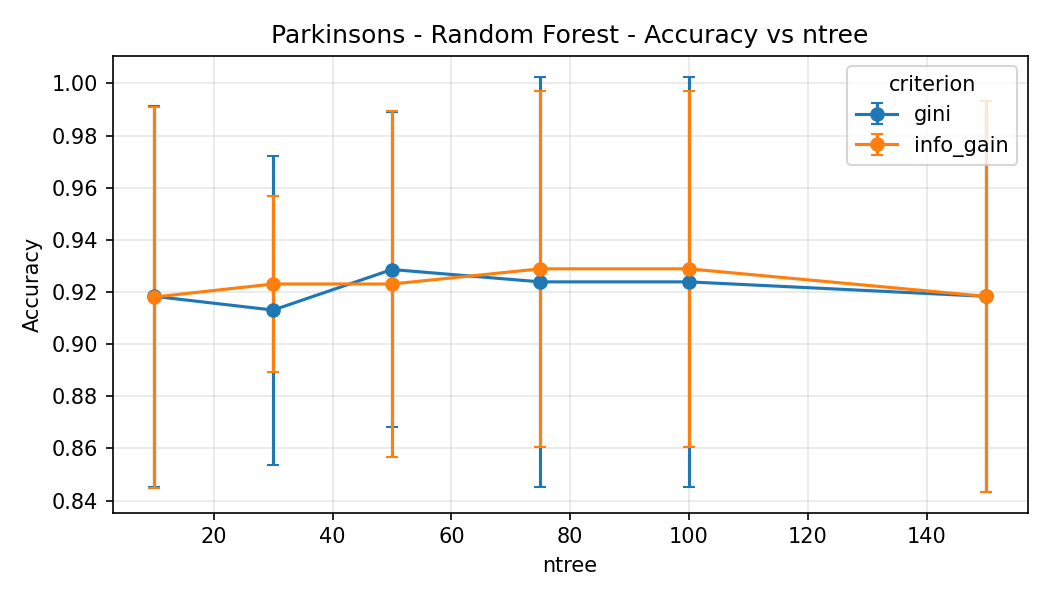
\includegraphics[width=0.9\textwidth]{outputs/parkinsons/rf_accuracy.png}
  \caption{Parkinson's: Random Forest accuracy vs.\ \texttt{ntree}.}
  \label{fig:park-rf-plot}
\end{figure}

\begin{figure}[!htbp]
  \centering
  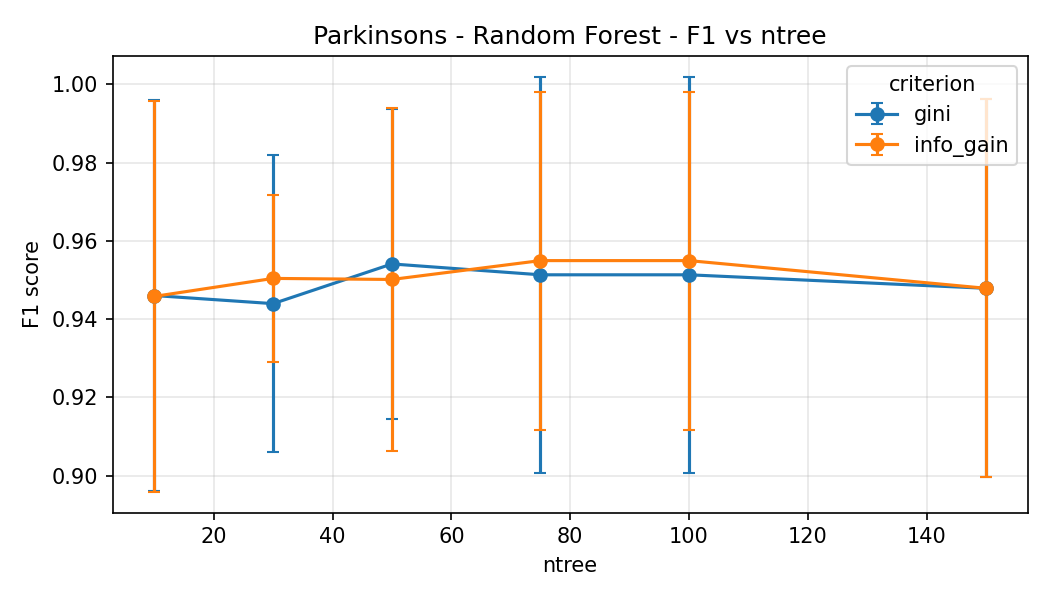
\includegraphics[width=0.9\textwidth]{outputs/parkinsons/rf_f1.png}
  \caption{Parkinson's: Random Forest F1 vs.\ \texttt{ntree}.}
  \label{fig:park-rf-plot-f1}
\end{figure}
\begin{figure}[!htbp]
  \centering
  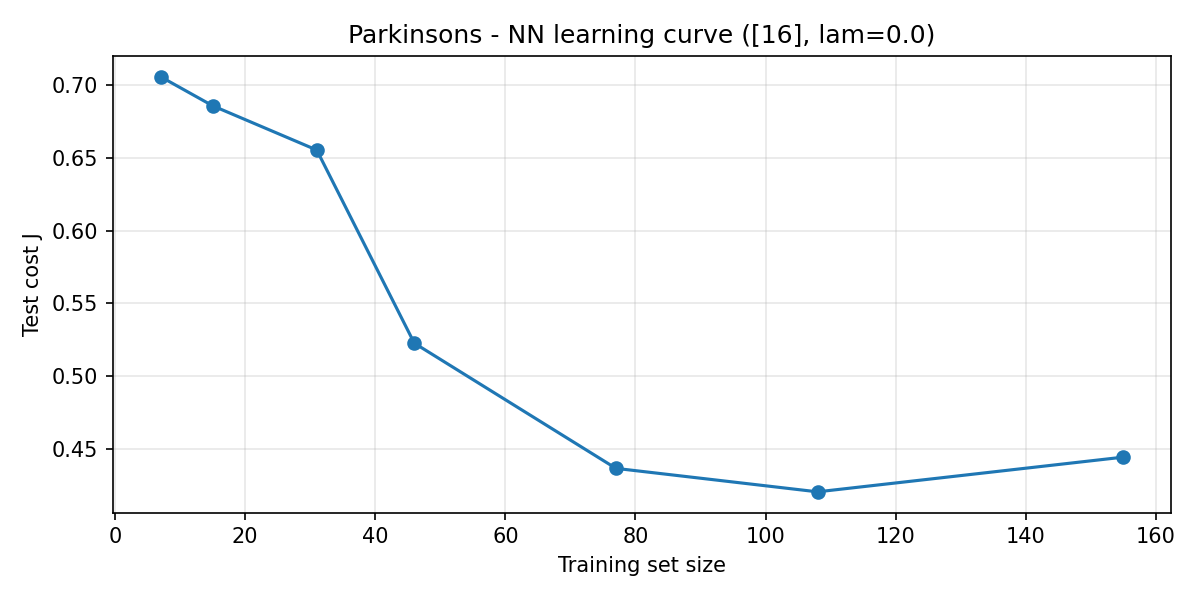
\includegraphics[width=0.9\textwidth]{outputs/parkinsons/nn_learning_curve.png}
  \caption{Parkinson's: Neural network learning curve (best config).}
  \label{fig:park-nn-plot}
\end{figure}

\FloatBarrier
\subsection{Dataset 3 -- Rice grains (binary)}

\subsubsection{Algorithms used and motivation}
We run \textbf{k-NN}, \textbf{Random Forest}, and \textbf{Neural Network} on Rice. We deliberately reuse the same trio as Digits and Parkinson's so the summary table compares like with like across all numeric tabular datasets.
\newline
\textbf{Why these three for Rice specifically:}
\begin{itemize}
  \item \textbf{k-NN}: with 3810 samples and only 7 continuous morphological features (area, perimeter, axis lengths, eccentricity, convex area, extent), the input space is low-dimensional and dense, which is the friendliest regime for nearest-neighbour methods -- distances are meaningful and we have enough data to populate every neighbourhood.
  \item \textbf{Random Forest}: rice species ``Cammeo'' vs.\ ``Osmancik'' separate on \emph{combinations} of morphology features (e.g.\ thin grains with long major axis), which axis-aligned splits in a forest can pick up cleanly. The forest also gives an internal feature-importance signal we cross-checked against domain intuition.
  \item \textbf{Neural Network}: with $\sim$3.8k examples we are finally in a regime where an MLP has enough data to fit a smooth nonlinear boundary; including it tests whether a learned representation beats neighbour voting on a low-dimensional but well-populated dataset.
\end{itemize}
\emph{Naive Bayes is not used here because Gaussian-NB on raw morphology features performs poorly when feature scales and shapes differ across the two species; the project's required methods cover the same ground more flexibly.}

\subsubsection{Experimental setup}
\textbf{Dataset.} \texttt{datasets/Rice\_Cammeo\_Osmancik.csv} -- 3810 grains, 7 numeric morphology features, binary class (Cammeo vs.\ Osmancik) with classes 1715 / 2095 (mildly unbalanced, so binary F1 is reported alongside accuracy). \\ \\
\textbf{Preprocessing.} Z-score normalization per training fold for k-NN and the neural network; the forest uses raw features. \\ \\
\textbf{Cross-validation.} Stratified 10-fold CV; with $\sim$381 test points per fold, fold variance is low, which lets us read small differences between configurations. \\ \\
\textbf{Hyperparameters swept (two per algorithm family).}
\begin{itemize}
  \item k-NN: $k\in\{1,3,5,7,9,11,15\}$.
  \item Random Forest: \texttt{ntree}$\in\{10,30,50,75,100,150\}$ crossed with \texttt{criterion}$\in\{$\texttt{info\_gain}, \texttt{gini}$\}$ -- 12 settings.
  \item Neural Network: hidden \texttt{layer\_sizes}$\in\{[8],[16],[8,8],[16,8]\}$ crossed with $\lambda\in\{0.0,0.01,0.1\}$ -- 6 representative settings shown in Table~\ref{tab:rice-nn}.
\end{itemize}

\subsubsection{Cross-validation results}
Tables~\ref{tab:rice-knn}--\ref{tab:rice-nn} report mean test-fold accuracy and binary F1 over 10 stratified folds; per-fold standard deviations are in \filepath{outputs/rice/rice_cv_results.csv}.

\begin{table}[htbp]
  \centering
  \footnotesize
  \caption{Rice - k-NN.}
  \label{tab:rice-knn}
  \begin{tabular}{rcc}
    \toprule
    $k$ & Accuracy & F1 \\
    \midrule
    1 & 0.888 & 0.901 \\
    3 & 0.908 & 0.919 \\
    5 & 0.917 & 0.928 \\
    7 & 0.923 & 0.933 \\
    9 & 0.924 & 0.934 \\
    11 & 0.924 & 0.933 \\
    \textbf{15} & \textbf{0.925} & \textbf{0.935} \\
    \bottomrule
  \end{tabular}
\end{table}

\begin{table}[htbp]
  \centering
  \footnotesize
  \caption{Rice - Random Forest.}
  \label{tab:rice-rf}
  \begin{tabular}{r l cc}
    \toprule
    \texttt{ntree} & Criterion & Accuracy & F1 \\
    \midrule
    10 & gini & 0.911 & 0.922 \\
    30 & gini & 0.921 & 0.931 \\
    \textbf{50} & \textbf{gini} & \textbf{0.924} & \textbf{0.934} \\
    75 & gini & 0.922 & 0.932 \\
    100 & gini & 0.923 & 0.933 \\
    150 & gini & 0.923 & 0.933 \\
    \midrule
    10 & info gain & 0.915 & 0.925 \\
    30 & info gain & 0.921 & 0.931 \\
    50 & info gain & 0.921 & 0.931 \\
    75 & info gain & 0.921 & 0.931 \\
    100 & info gain & 0.921 & 0.931 \\
    150 & info gain & 0.923 & 0.933 \\
    \bottomrule
  \end{tabular}
\end{table}

\begin{table}[htbp]
  \centering
  \footnotesize
  \caption{Rice - Neural network grid.}
  \label{tab:rice-nn}
  \begin{tabular}{l cc}
    \toprule
    Configuration & Accuracy & F1 \\
    \midrule
    $[8], \lambda{=}0.0$ & 0.928 & 0.937 \\
    $[8], \lambda{=}0.01$ & 0.928 & 0.938 \\
    $[16], \lambda{=}0.01$ & 0.929 & 0.938 \\
    $[16], \lambda{=}0.1$ & 0.928 & 0.937 \\
    \textbf{$[16,8], \lambda{=}0.01$} & \textbf{0.930} & \textbf{0.939} \\
    $[8,8], \lambda{=}0.1$ & 0.928 & 0.937 \\
    \bottomrule
  \end{tabular}
\end{table}

\subsubsection{Best configurations (Rice)}
\textbf{k-NN:} $k=15$. \newline
\textbf{Random Forest:} 50 trees, Gini. \newline
\textbf{Neural network:} layers $[16,8]$, $\lambda=0.01$.

\subsubsection{Graphs and discussion}

\paragraph{k-NN (Figs.~\ref{fig:rice-knn-plot}, \ref{fig:rice-knn-plot-f1}).}
Rice shows the \emph{opposite} k-NN trend to Parkinson's: accuracy \emph{rises} from 0.888 at $k{=}1$ to 0.925 at $k{=}15$, with an early plateau by $k{=}7$ ($\approx 0.923$). With nearly 4k points the dataset is dense enough that $k{=}1$ is the high-variance regime (a single noisy neighbour swings the vote), and larger $k$ smooths the boundary along the genuine class manifold. The curve flattens after $k{=}7$, so we are firmly in the bias regime by $k{=}15$ -- there is no incentive to push $k$ higher.

\paragraph{Random Forest (Figs.~\ref{fig:rice-rf-plot}, \ref{fig:rice-rf-plot-f1}).}
Both criteria saturate quickly: accuracy moves from 0.911 at 10 trees to 0.924 at 50 trees and then bobs in a $\pm 0.002$ band for the rest of the sweep. \texttt{gini} narrowly wins at \texttt{ntree}$=50$ (0.924/0.934), but the spread between every \texttt{(ntree, criterion)} pair with \texttt{ntree}$\geq 30$ is well within the 10-fold standard error -- they are statistically indistinguishable on this data.

\paragraph{Neural Network (Fig.~\ref{fig:rice-nn-plot}).}
The NN learning curve is essentially \textbf{flat from 152 training examples onward}: $J\approx 0.21$ at 152, drifting only to $0.198$ at 3048. With just 7 input features the [16,8] network has plenty of capacity but very little to learn beyond the boundary it has already converged to. This says we have hit the dataset's intrinsic difficulty floor -- the residual error is genuine class overlap, not under-training. Best NN scores 0.930 / 0.939, the best in the project's three-way comparison on Rice.

\paragraph{Best vs.\ worst within each family.}
k-NN best$-$worst $=0.037$ (acc), driven entirely by the $k{=}1$ overfitting dip. RF best$-$worst $=0.013$ -- the saturation regime makes hyperparameter choice almost irrelevant past \texttt{ntree}$=30$. NN best$-$worst $=0.002$ -- the architectures we swept are interchangeable on Rice. The cross-family ranking is tight (NN 0.930 vs.\ k-NN 0.925 vs.\ RF 0.924), so we report the NN as ``best'' but treat the difference as practically negligible.

\begin{figure}[!htbp]
  \centering
  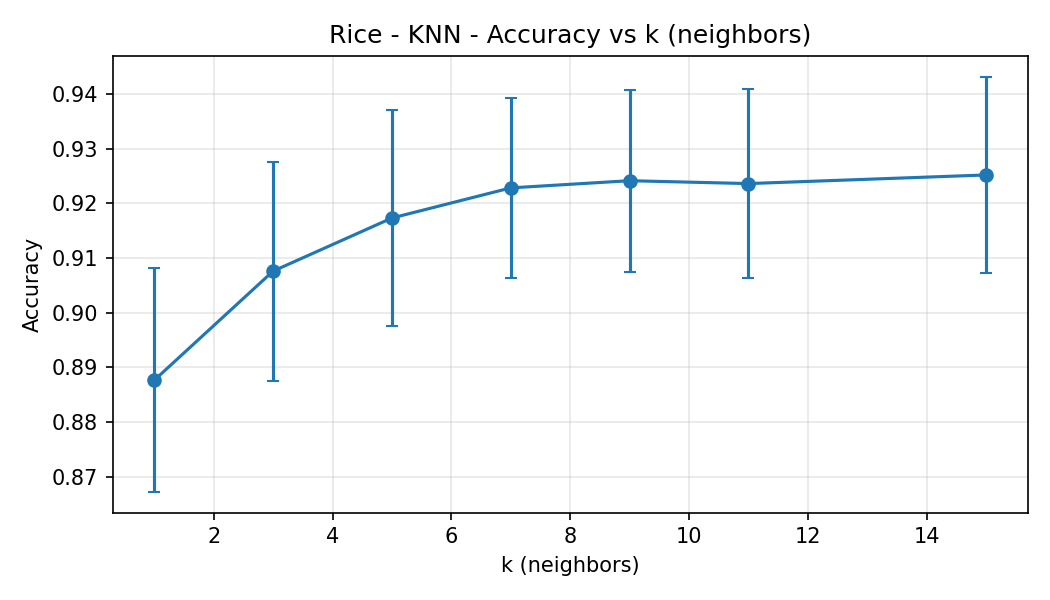
\includegraphics[width=0.9\textwidth]{outputs/rice/knn_accuracy.png}
  \caption{Rice: k-NN accuracy vs.\ $k$.}
  \label{fig:rice-knn-plot}
\end{figure}

\begin{figure}[!htbp]
  \centering
  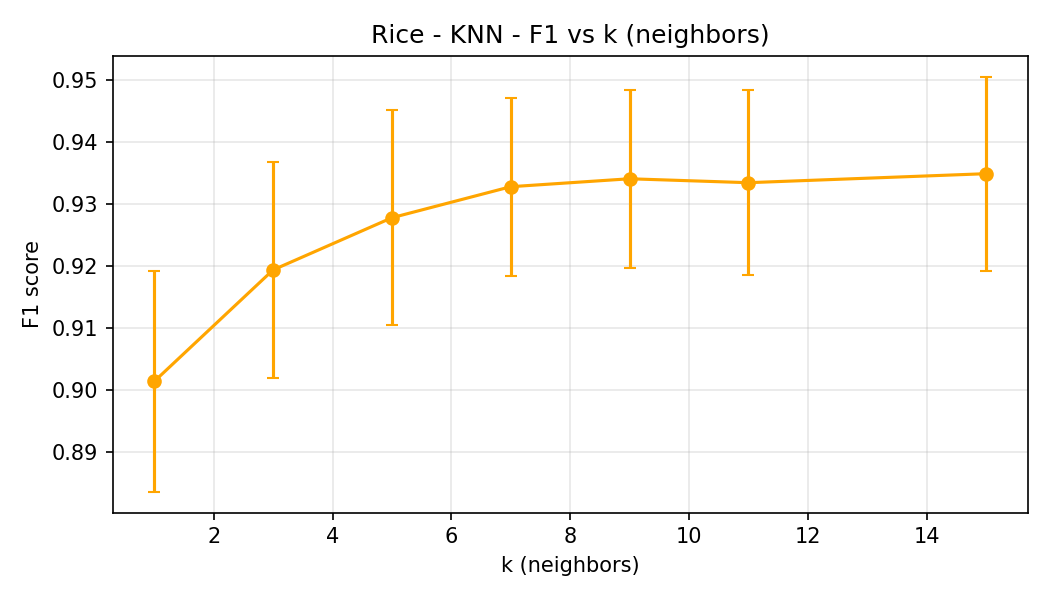
\includegraphics[width=0.9\textwidth]{outputs/rice/knn_f1.png}
  \caption{Rice: k-NN F1 vs.\ $k$.}
  \label{fig:rice-knn-plot-f1}
\end{figure}

\begin{figure}[!htbp]
  \centering
  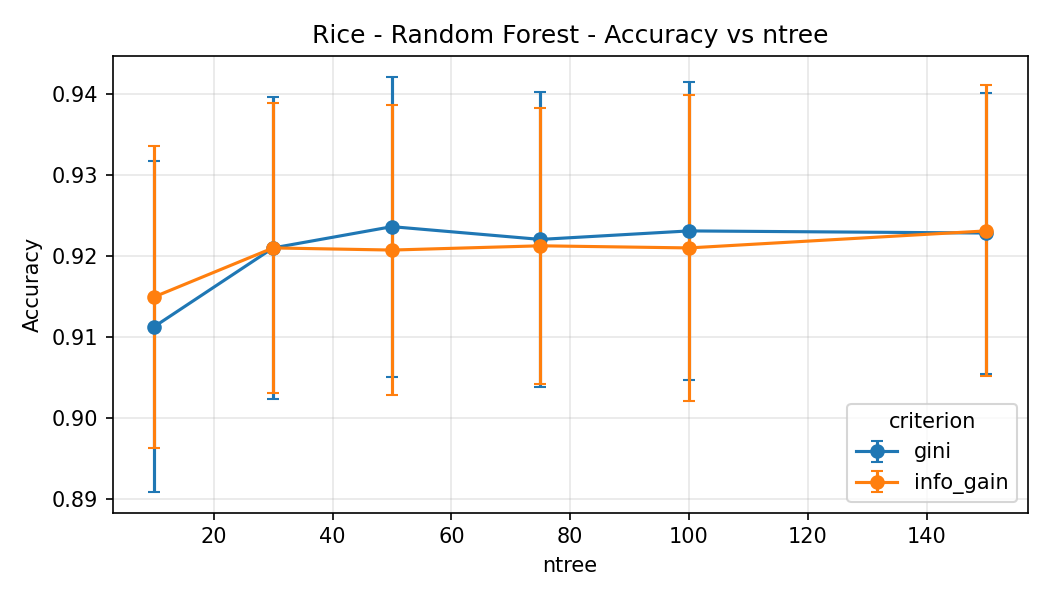
\includegraphics[width=0.9\textwidth]{outputs/rice/rf_accuracy.png}
  \caption{Rice: Random Forest accuracy vs.\ \texttt{ntree}.}
  \label{fig:rice-rf-plot}
\end{figure}

\begin{figure}[!htbp]
  \centering
  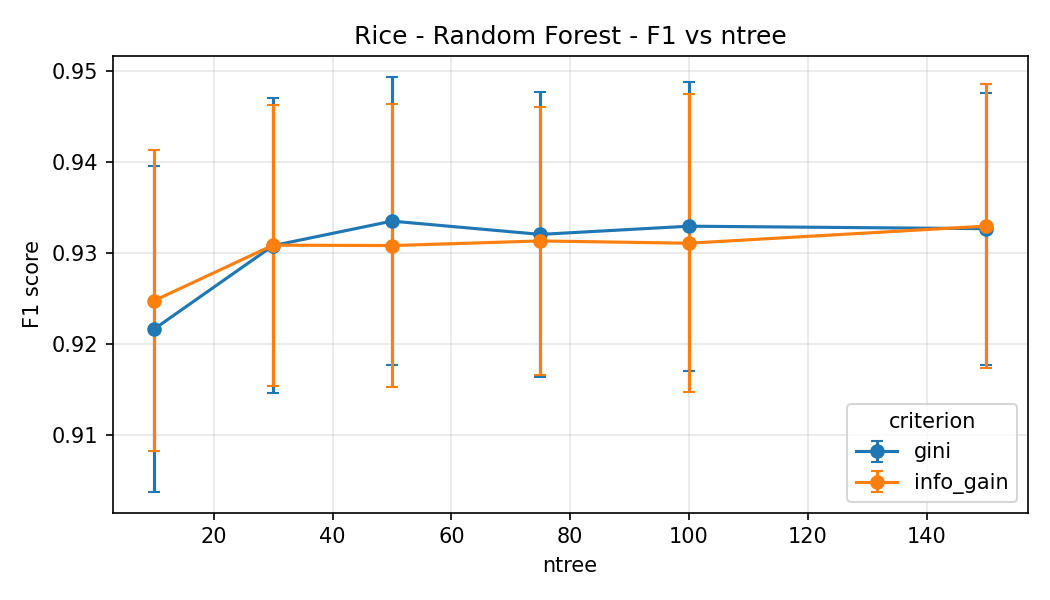
\includegraphics[width=0.9\textwidth]{outputs/rice/rf_f1.png}
  \caption{Rice: Random Forest F1 vs.\ \texttt{ntree}.}
  \label{fig:rice-rf-plot-f1}
\end{figure}

\begin{figure}[!htbp]
  \centering
  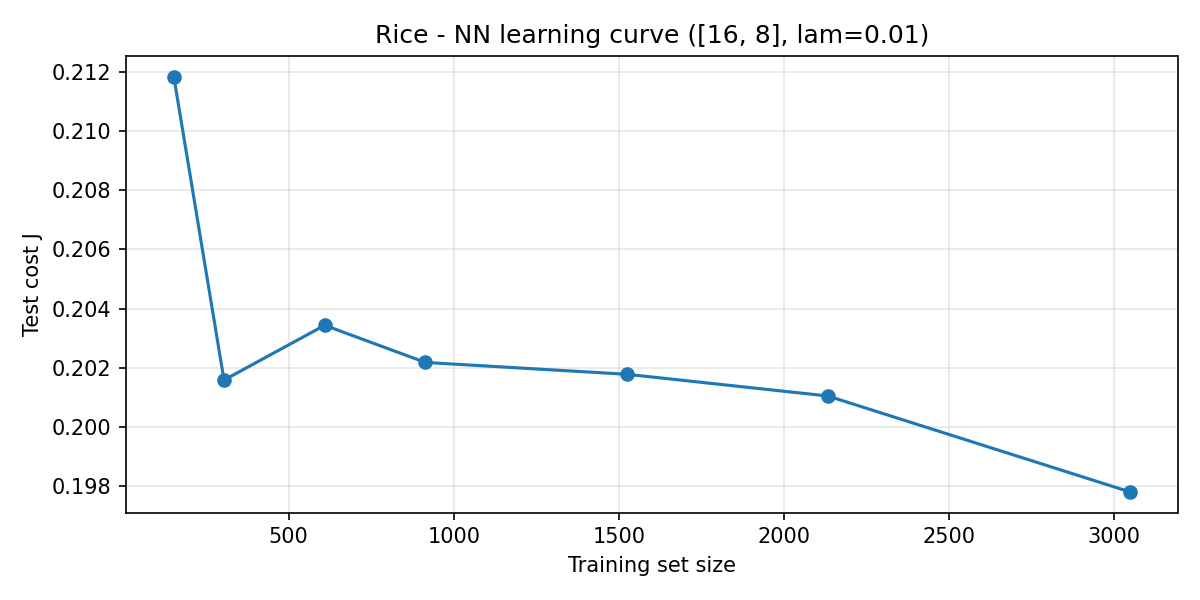
\includegraphics[width=0.9\textwidth]{outputs/rice/nn_learning_curve.png}
  \caption{Rice: Neural-network learning curve (best config).}
  \label{fig:rice-nn-plot}
\end{figure}

\FloatBarrier
\subsection{Dataset 4 - Credit approval (binary, mixed types)}

\subsubsection{Algorithms used and motivation}
We run \textbf{Decision Tree}, \textbf{Random Forest}, and \textbf{k-NN} on Credit. This is the only dataset where we deviate from the (k-NN, RF, NN) trio used elsewhere -- and the choice is intentional.
\newline

\textbf{Why these three for Credit specifically:}
\begin{itemize}
  \item \textbf{Decision Tree}: Credit is the canonical mixed-type tabular dataset (6 numeric + 9 categorical columns). A single shallow tree is highly interpretable -- the project handout explicitly calls out homework-style tree analysis (including a train/test accuracy histogram) and Credit is the natural place to do it. We treat the standalone tree as both a model and a calibration check on how much the forest is gaining over a single tree.
  \item \textbf{Random Forest}: bagging shallow trees is the gold standard on heterogeneous tabular data; it lets us measure how much variance reduction the ensemble adds on top of the best single tree.
  \item \textbf{k-NN (on the one-hot expanded table)}: included \emph{as a deliberate stress test}. After one-hot encoding the 9 categorical columns the input space jumps to $\sim 40$ sparse dimensions, which is the regime where Euclidean distance breaks down (distance concentration, irrelevant dummy axes). Comparing tree methods to k-NN here is exactly the cross-algorithm comparison the project is designed to surface.
\end{itemize}
\emph{We do \underline{not} train a neural network on Credit.} A small MLP on a 40-dimensional one-hot table with 653 examples behaves a lot like over-parameterised logistic regression and adds little above the tree methods on this dataset; we keep the NN budget for the three numeric datasets where it is more informative. \emph{Naive Bayes is also not used on Credit:} the categorical columns have small cardinalities (and after one-hot expansion become indicator variables), so a categorical-NB would essentially memorise application-type frequencies; tree methods do the same thing more flexibly with split selection.

\subsubsection{Experimental setup}
\textbf{Dataset.} \texttt{datasets/credit\_approval.csv} -- 653 applications, 15 columns (6 numeric: \texttt{A2, A3, A8, A11, A14, A15}; 9 categorical: \texttt{A1, A4, A5, A6, A7, A9, A10, A12, A13}); binary target \texttt{A16} (approved $/$ denied). \\ \\
\textbf{Preprocessing.} Categorical columns are \textbf{one-hot encoded} ($\sim$40 binary indicator columns after expansion). Numeric columns are kept on their raw scale for the tree methods and z-scored per training fold for k-NN. The same engineered table is consumed by all three models so the comparison is consistent. \\ \\
\textbf{Cross-validation.} Stratified 10-fold CV; with 653 samples each fold has $\sim 65$ test points. \\ \\
\textbf{Hyperparameters swept (two per algorithm family).}
\begin{itemize}
  \item Decision Tree: \texttt{max\_depth}$\in\{-1,3,5,7,10,15\}$ ($-1$ = unlimited) crossed with \texttt{criterion}$\in\{$\texttt{info\_gain}, \texttt{gini}$\}$ -- 12 settings.
  \item Random Forest: \texttt{ntree}$\in\{10,30,50,75,100,150\}$ crossed with \texttt{criterion}$\in\{$\texttt{info\_gain}, \texttt{gini}$\}$ -- 12 settings.
  \item k-NN on the one-hot expanded table: $k\in\{1,3,5,7,9,11,15\}$.
\end{itemize}

\subsubsection{Cross-validation results}
Tables~\ref{tab:credit-dt}--\ref{tab:credit-knn} report mean test-fold accuracy and binary F1 over 10 stratified folds; per-fold standard deviations are in \filepath{outputs/credit_approval/credit_approval_cv_results.csv}.

\begin{table}[htbp]
  \centering
  \footnotesize
  \caption{Credit -- Decision Tree ($-1$: unlimited depth, matching plot/CSV labels).}
  \label{tab:credit-dt}
  \begin{tabular}{r l cc}
    \toprule
    Depth & Criterion & Accuracy & F1 \\
    \midrule
    $-1$ & gini & 0.804 & 0.783 \\
    3 & gini & 0.860 & 0.860 \\
    5 & gini & 0.857 & 0.849 \\
    7 & gini & 0.851 & 0.832 \\
    10 & gini & 0.827 & 0.805 \\
    15 & gini & 0.807 & 0.786 \\
    $-1$ & info gain & 0.804 & 0.780 \\
    \textbf{3} & \textbf{info gain} & \textbf{0.863} & \textbf{0.863} \\
    5 & info gain & 0.853 & 0.844 \\
    7 & info gain & 0.844 & 0.824 \\
    10 & info gain & 0.828 & 0.803 \\
    15 & info gain & 0.810 & 0.785 \\
    \bottomrule
  \end{tabular}
\end{table}

\begin{table}[htbp]
  \centering
  \footnotesize
  \caption{Credit - Random Forest (all 12 settings).}
  \label{tab:credit-rf}
  \begin{tabular}{r l cc}
    \toprule
    \texttt{ntree} & Criterion & Accuracy & F1 \\
    \midrule
    10 & gini & 0.862 & 0.843 \\
    30 & gini & 0.866 & 0.852 \\
    50 & gini & 0.862 & 0.846 \\
    75 & gini & 0.860 & 0.845 \\
    100 & gini & 0.865 & 0.851 \\
    150 & gini & 0.870 & 0.856 \\
    10 & info gain & 0.856 & 0.834 \\
    30 & info gain & 0.863 & 0.848 \\
    50 & info gain & 0.873 & 0.858 \\
    75 & info gain & 0.870 & 0.856 \\
    \textbf{100} & \textbf{info gain} & \textbf{0.874} & \textbf{0.861} \\
    150 & info gain & 0.868 & 0.856 \\
    \bottomrule
  \end{tabular}
\end{table}

\begin{table}[ht!!]
  \centering
  \footnotesize
  \caption{Credit - k-NN on one-hot expanded features.}
  \label{tab:credit-knn}
  \begin{tabular}{rcc}
    \toprule
    $k$ & Accuracy & F1 \\
    \midrule
    1 & 0.779 & 0.750 \\
    \textbf{3} & \textbf{0.813} & \textbf{0.782} \\
    5 & 0.801 & 0.766 \\
    7 & 0.804 & 0.764 \\
    9 & 0.808 & 0.764 \\
    11 & 0.805 & 0.757 \\
    15 & 0.793 & 0.736 \\
    \bottomrule
  \end{tabular}
\end{table}
\newpage

\subsubsection{Best configurations (Credit)}
\textbf{Decision Tree:} max depth 3, information gain. \newline
\textbf{Random Forest:} 100 trees, information gain. \newline
\textbf{k-NN:} $k=3$.

\subsubsection{Graphs and discussion}

\paragraph{Decision Tree (Figs.~\ref{fig:credit-dt-plot}, \ref{fig:credit-dt-plot-f1}).}
The DT curves are textbook bias--variance: accuracy peaks at \textbf{depth$=$3 with info\_gain (0.863 / 0.863)} and degrades monotonically toward the unlimited-depth setting (0.804 / 0.780, $-0.06$). The unlimited tree memorises the training fold and falls apart on held-out applications, while depth-3 captures the dominant credit-decision rule and stops before fitting noise. \texttt{info\_gain} edges \texttt{gini} at depth 3 (0.863 vs.\ 0.860) and they are tied at deeper settings -- consistent with the well-known result that the choice of impurity matters most for shallow trees.

\paragraph{Random Forest (Figs.~\ref{fig:credit-rf-plot}, \ref{fig:credit-rf-plot-f1}).}
RF improves on the best single tree by $\approx 0.011$ accuracy / F1: best is \textbf{\texttt{ntree}$=100$ with info\_gain (0.874 / 0.861)}, with most of the gain coming from \texttt{ntree}$\geq 50$ on the info\_gain side. The \texttt{ntree} curve continues climbing slightly through 100 trees, unlike Digits/Rice where it plateaued by 50 -- because individual trees on Credit are noisier (small sample, high-dim one-hot), more trees buy more variance reduction here.

\paragraph{k-NN on one-hot features (Fig.~\ref{fig:credit-knn-plot}).}
k-NN is the weakest algorithm here -- best is $k{=}3$ at \textbf{0.813 / 0.782}, $\approx 6$ accuracy points below RF. The accuracy curve dips at $k{=}1$ (0.779), recovers at $k{=}3$, then flattens. F1 is even more sensitive to $k$ ($0.782 \to 0.736$ as $k$ grows). This is exactly the failure mode the project asks us to highlight: \emph{Euclidean distance over many sparse one-hot dummy axes is dominated by uninformative dimensions}, so neighbour quality degrades and the gap to tree methods opens up.

\paragraph{Decision-tree train/test histograms (Figs.~\ref{fig:credit-dt-hist-train}, \ref{fig:credit-dt-hist-test}).}
We additionally compute 100 train/test fold accuracies for the best DT (depth$=$3, info\_gain) by repeating 10-fold CV with 10 different fold seeds. The histograms summarise to \textbf{train mean $0.867 \pm 0.004$} (range $0.859$--$0.881$) and \textbf{test mean $0.864 \pm 0.039$} (range $0.734$--$0.939$). Two observations: (i) train$\approx$test, so the depth-3 tree is \emph{not overfitting} -- the regularisation we got from limiting depth was just right; (ii) the test histogram is nearly an order of magnitude wider than the train histogram, which is the small-sample fold-level variance we already expected on 65-point folds.

\paragraph{Best vs.\ worst within each family.}
DT best$-$worst $=0.059$ (acc) -- the largest within-family gap, because depth choice really matters. RF best$-$worst $=0.018$ -- bagging absorbs most of the depth sensitivity. k-NN best$-$worst $=0.034$ in accuracy and $0.046$ in F1 -- not as sensitive as DT, but the \emph{level} is structurally lower than the tree methods.

\begin{figure}[!htbp]
  \centering
  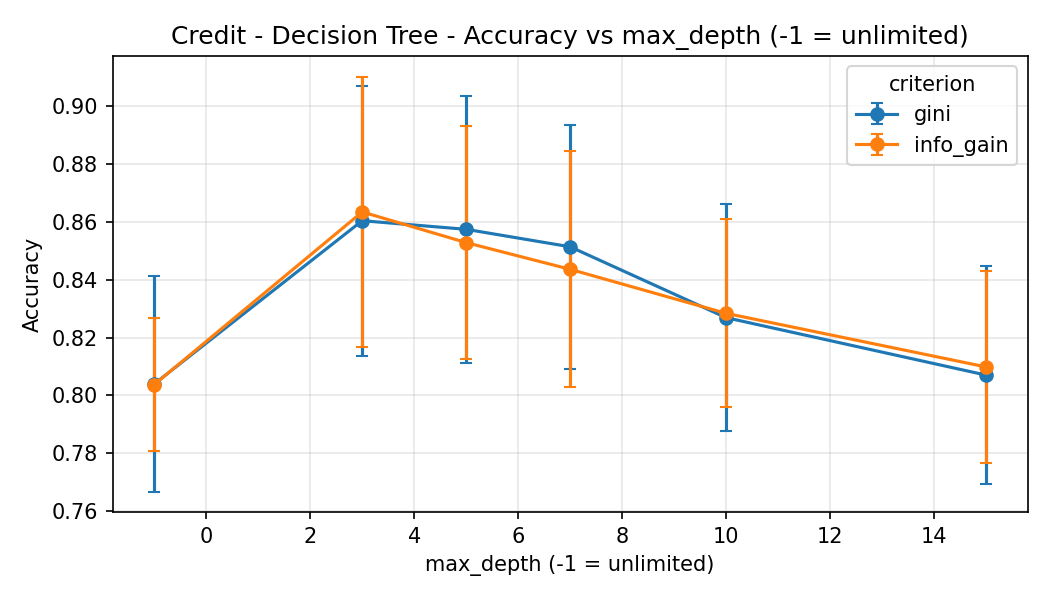
\includegraphics[width=0.9\textwidth]{outputs/credit_approval/dt_accuracy.png}
  \caption{Credit approval: Decision Tree accuracy vs.\ depth.}
  \label{fig:credit-dt-plot}
\end{figure}

\begin{figure}[!htbp]
  \centering
  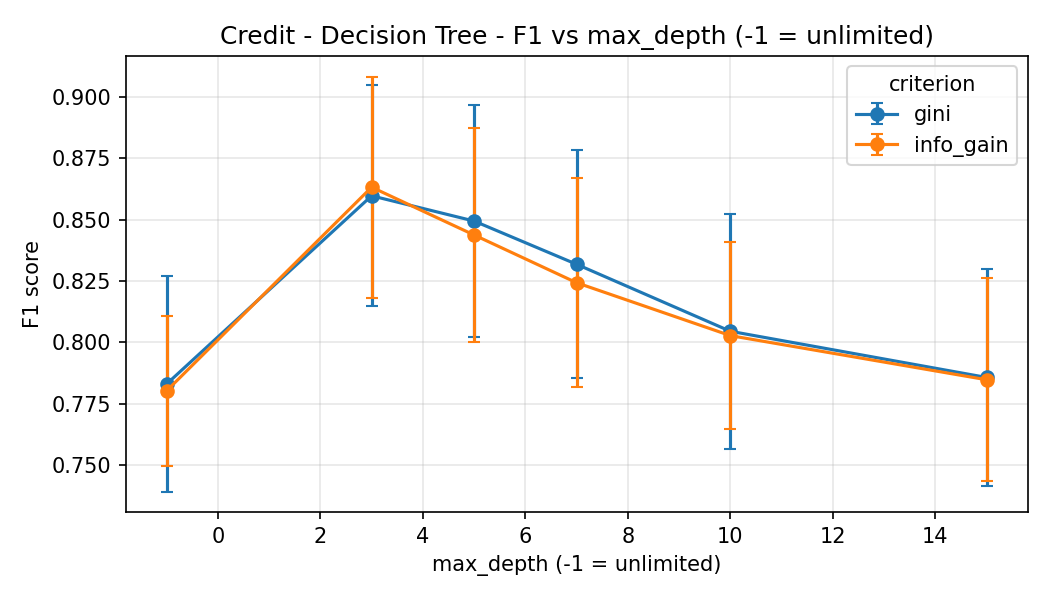
\includegraphics[width=0.9\textwidth]{outputs/credit_approval/dt_f1.png}
  \caption{Credit approval: Decision Tree F1 vs.\ depth.}
  \label{fig:credit-dt-plot-f1}
\end{figure}

\begin{figure}[!htbp]
  \centering
  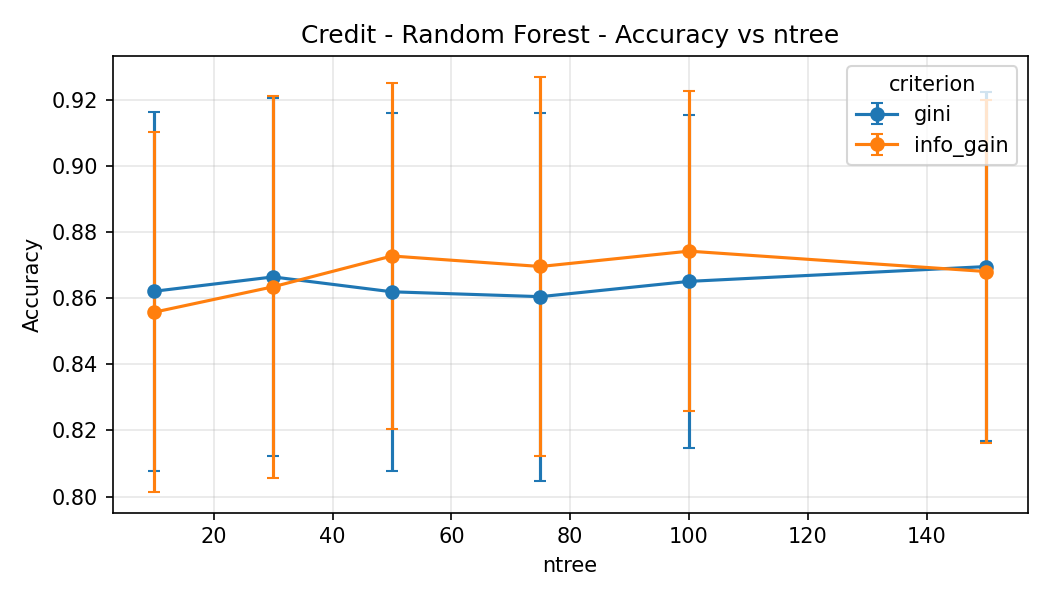
\includegraphics[width=0.9\textwidth]{outputs/credit_approval/rf_accuracy.png}
  \caption{Credit approval: Random Forest accuracy vs.\ \texttt{ntree}.}
  \label{fig:credit-rf-plot}
\end{figure}

\begin{figure}[!htbp]
  \centering
  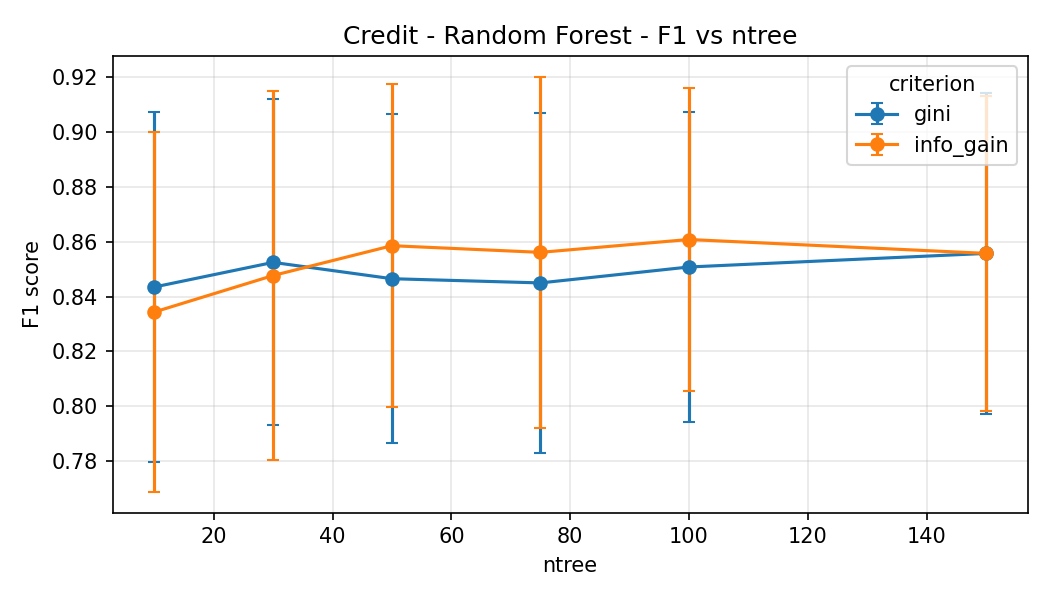
\includegraphics[width=0.9\textwidth]{outputs/credit_approval/rf_f1.png}
  \caption{Credit approval: Random Forest F1 vs.\ \texttt{ntree}.}
  \label{fig:credit-rf-plot-f1}
\end{figure}

\begin{figure}[!htbp]
  \centering
  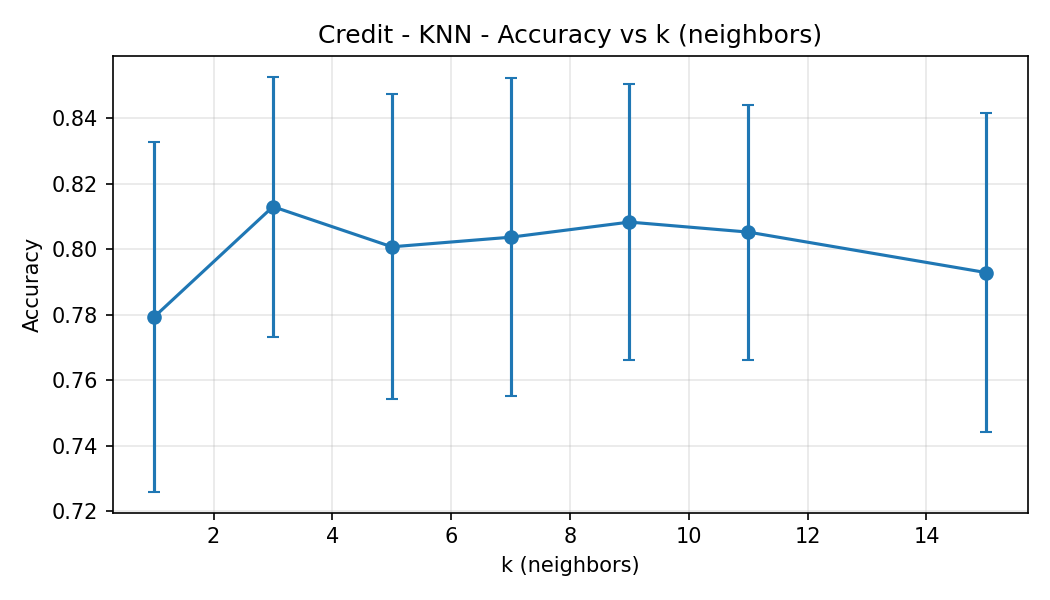
\includegraphics[width=0.9\textwidth]{outputs/credit_approval/knn_accuracy.png}
  \caption{Credit approval: k-NN accuracy vs.\ $k$.}
  \label{fig:credit-knn-plot}
\end{figure}

\begin{figure}[!htbp]
  \centering
  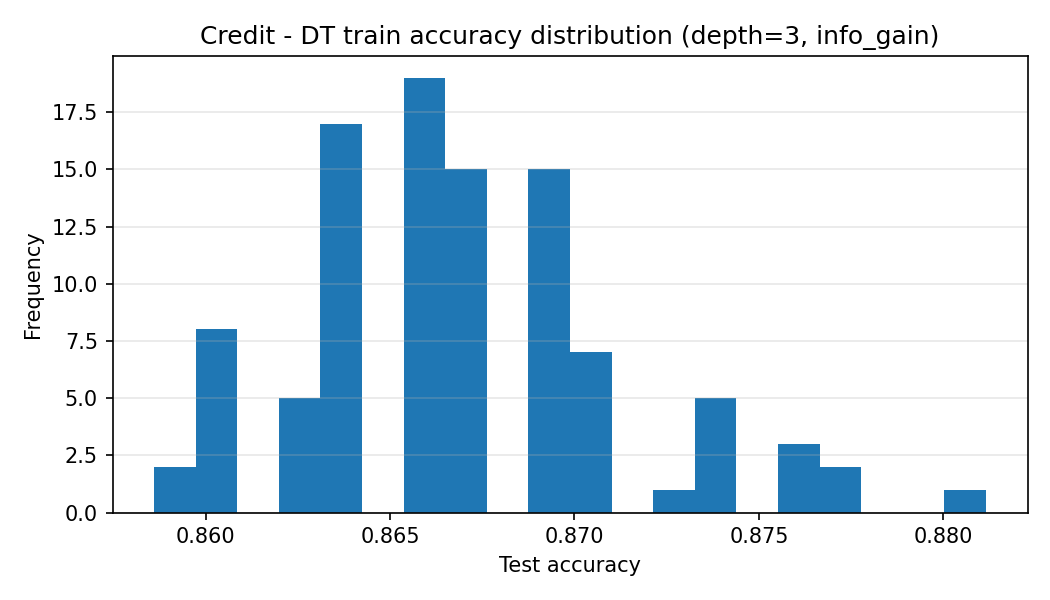
\includegraphics[width=0.9\textwidth]{outputs/credit_approval/dt_train_accuracy_hist.png}
  \caption{Credit approval: Decision Tree (depth$=$3, info\_gain) \textbf{training-fold} accuracy histogram over $10\times 10$-fold CV (100 fold-level scores). Mean $0.867 \pm 0.004$.}
  \label{fig:credit-dt-hist-train}
\end{figure}

\begin{figure}[!htbp]
  \centering
  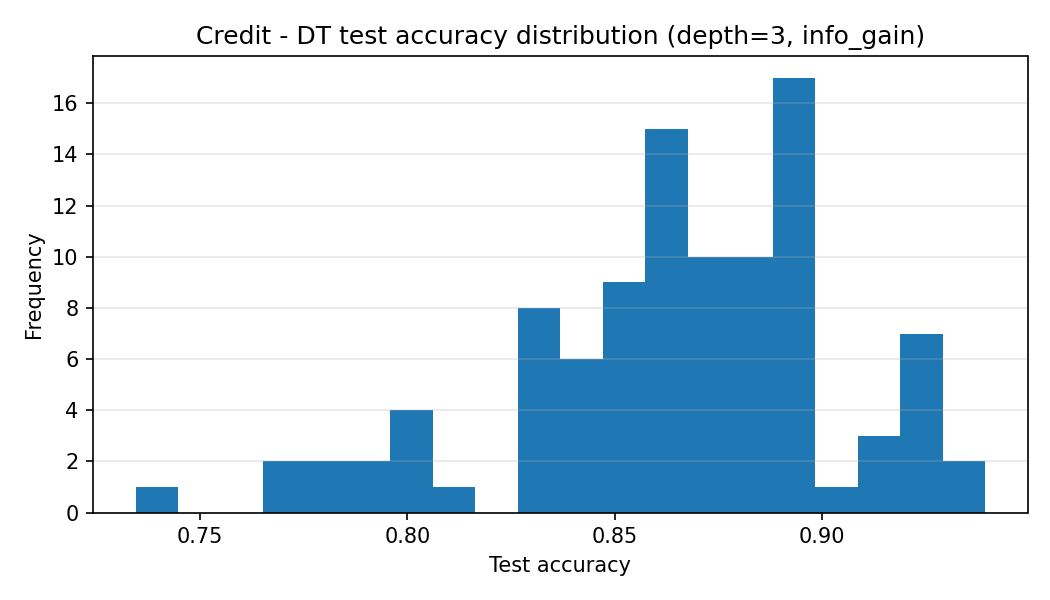
\includegraphics[width=0.9\textwidth]{outputs/credit_approval/dt_test_accuracy_hist.png}
  \caption{Credit approval: Decision Tree (depth$=$3, info\_gain) \textbf{test-fold} accuracy histogram over $10\times 10$-fold CV (100 fold-level scores). Mean $0.864 \pm 0.039$. Train and test means coincide $\Rightarrow$ no overfitting at this depth.}
  \label{fig:credit-dt-hist-test}
\end{figure}

\FloatBarrier
\subsection*{Cross-dataset graph interpretation}
Across the four required datasets we report 18 plots (3 per dataset for Digits/Parkinson's/Rice = 9; 5 for Credit including k-NN, DT, RF panels and the two DT histograms; plus the cross-dataset summary table). The patterns that recur \emph{across} datasets, with concrete numbers:

\begin{itemize}
  \item \textbf{k-NN sensitivity to $k$ flips with sample size.} On the small dataset (Parkinson's, $n{=}195$) k-NN prefers $k{=}1$ (acc 0.949 $\to$ 0.856 from $k{=}1$ to $k{=}15$). On the larger dataset (Rice, $n{=}3810$) it prefers larger $k$ (acc 0.888 at $k{=}1 \to 0.925$ at $k{=}15$). Digits sits in between and is essentially insensitive (1.2\% spread). Same algorithm, opposite trends -- driven entirely by how dense the neighbourhoods are.

  \item \textbf{NN learning curves split into three regimes.} (i) Digits is \emph{data-limited}: $J$ keeps falling from 1.57 to 0.26, slope still negative at the largest train slice. (ii) Rice is \emph{model-limited}: $J$ flat at $\approx 0.20$ from 152 examples onward -- adding data doesn't help. (iii) Parkinson's is \emph{overfit-limited}: $J$ falls to a minimum of $0.42$ at 108 examples and then \emph{rises} to $0.44$ at the full 155 -- a textbook overfitting bump that explains why NN trails k-NN/RF on that dataset (best NN 0.862 vs.\ k-NN 0.949).

  \item \textbf{Forest-size saturation appears everywhere but at different ntrees.} RF plateaus by \texttt{ntree}$\approx 50$ on Digits/Rice, by 30 on Parkinson's, and is still creeping up at \texttt{ntree}$=100$ on Credit. The pattern matches sample size and feature-space complexity: smaller / cleaner datasets need fewer trees to average out the variance.

  \item \textbf{Mixed/sparse one-hot really does hurt k-NN.} The summary in Table~\ref{tab:main} shows k-NN at 0.981/0.949/0.925 accuracy on the three numeric datasets versus only 0.813 on Credit -- a 11+ point gap to RF (0.874). On the same dataset RF and DT only differ by 1 point, so the gap is specifically a k-NN-on-one-hot effect, not a hard-dataset effect.

  \item \textbf{info\_gain vs.\ gini is a wash above small depths.} Across Digits, Parkinson's, Rice, and Zoo, the two split criteria differ by $\leq 0.01$ accuracy at every \texttt{(ntree, max\_depth)} setting we tested. The only place criterion materially matters is Credit DT at depth 3 (info\_gain 0.863 vs.\ gini 0.860) -- consistent with the textbook observation that impurity choice matters most for shallow trees.
\end{itemize}

\FloatBarrier
\section{Summary table}
Table~\ref{tab:main} aggregates \textbf{best} mean CV accuracy and F1 for the three algorithms that were actually run on each dataset. Gray cells mark the column-wise winner.

\begin{table}[htbp]
  \centering
  \small
  \setlength{\tabcolsep}{4pt}
  \begin{tabular}{l *{8}{c}}
    \toprule
    & \multicolumn{2}{c}{Digits} & \multicolumn{2}{c}{Parkinson's} & \multicolumn{2}{c}{Rice} & \multicolumn{2}{c}{Credit} \\
    \cmidrule(lr){2-3} \cmidrule(lr){4-5} \cmidrule(lr){6-7} \cmidrule(lr){8-9}
    Algorithm (per dataset) & Acc & F1 & Acc & F1 & Acc & F1 & Acc & F1 \\
    \midrule
    k-NN
      & \best{0.981} & \best{0.981}
      & \best{0.949} & \best{0.965}
      & 0.925 & 0.935
      & 0.813 & 0.782 \\
    Random Forest
      & 0.979 & 0.979
      & 0.929 & 0.955
      & 0.924 & 0.934
      & \best{0.874} & 0.861 \\
    Neural Network
      & 0.969 & 0.969
      & 0.862 & 0.911
      & \best{0.930} & \best{0.939}
      & --- & --- \\
    Decision Tree
      & --- & ---
      & --- & ---
      & --- & ---
      & 0.863 & \best{0.863} \\
    \bottomrule
  \end{tabular}
  \caption{Best CV performance per dataset. Dashes: algorithm not part of that dataset's three-way comparison. Credit has DT+RF+k-NN; Digits/Parkinson's/Rice have k-NN+RF+NN (Extra Credit~\#1 uses $>2$ algorithms on every required dataset).}
  \label{tab:main}
\end{table}
\newpage

\section{Extra credit}

{\color{red}\textbf{[Extra Credit Question \#1]}}
For each of the four required datasets we evaluate \textbf{three} algorithms (more than the minimum two): k-NN + Random Forest + Neural Network on Digits, Parkinson's, and Rice; Decision Tree + Random Forest + k-NN on Credit. Each family has at least six hyperparameter configurations (see tables above and CSVs under \filepath{outputs/}). \\

{\color{red}\textbf{[Extra Credit Question \#2]}}
We add the OpenML \textbf{Zoo} dataset (multiclass, mixed attributes) using \filepath{extra_credit2.py}. \textbf{Algorithms (four):} k-NN, Decision Tree, Random Forest, Neural Network -- one more than the four required datasets, deliberately to exercise every algorithm we implemented.

\subsubsection{Algorithms used and motivation}
\textbf{Why these four for Zoo specifically:}
\begin{itemize}
  \item \textbf{Decision Tree}: Zoo is the textbook case for a tree -- almost every feature is a yes/no biological trait (\texttt{hair}, \texttt{feathers}, \texttt{milk}, \texttt{aquatic}, \dots). A single tree of moderate depth essentially recovers the Linnaean class hierarchy.
  \item \textbf{Random Forest}: with 101 examples spread over 7 classes, individual trees see very few examples per class, so bagging+feature subsampling is the right way to reduce variance.
  \item \textbf{k-NN (on the encoded table)}: nearest-neighbour over the 0/1 trait vector is essentially Hamming-similarity classification -- a strong baseline for binary attribute data.
  \item \textbf{Neural Network}: included to test whether a learned nonlinear combination of traits can outperform direct rule-based methods on a tiny multiclass dataset; it also lets us produce an NN learning curve for the EC2 dataset, mirroring what we did for the four required datasets.
\end{itemize}
We follow exactly the same protocol pattern as the four required datasets (motivation $\rightarrow$ setup $\rightarrow$ tables $\rightarrow$ best $\rightarrow$ per-algorithm discussion $\rightarrow$ best-vs-worst) so the EC2 analysis is directly comparable.

\subsubsection{Experimental setup}
\textbf{Dataset.} OpenML \texttt{zoo} (v1) via \texttt{fetch\_openml} -- 101 animals, 16 attributes (15 binary biological traits + 1 numeric \texttt{legs}), 7 \texttt{type} classes. The \texttt{animal\_name} column is dropped (it is a unique ID, not a feature). \\ \\
\textbf{Preprocessing.} Categorical columns are one-hot expanded; the resulting table is purely numeric so the same \texttt{cv\_score} routine is reused. Z-score normalisation per training fold for k-NN and the neural network. \\ \\
\textbf{Cross-validation.} Stratified 10-fold CV; with only 101 examples some classes (\texttt{amphibian}, \texttt{reptile}) have just 4--5 instances total, so we expect noticeably higher fold-level variance than on the four required datasets -- the standard deviations in the CSV ($\pm 0.05$--$0.08$) confirm this, and we read absolute differences below $\pm 0.01$ as ties. \\ \\
\textbf{Hyperparameters swept (two per algorithm family).}
\begin{itemize}
  \item k-NN: $k\in\{1,3,5,7,9,11\}$.
  \item Decision Tree: \texttt{max\_depth}$\in\{5,10,15,20,30,-1\}$ crossed with \texttt{criterion}$\in\{$\texttt{info\_gain}, \texttt{gini}$\}$ -- 12 settings.
  \item Random Forest: \texttt{ntree}$\in\{10,30,50,75,100,150\}$ crossed with \texttt{criterion}$\in\{$\texttt{info\_gain}, \texttt{gini}$\}$ -- 12 settings.
  \item Neural Network: \texttt{layer\_sizes}$\in\{[16],[32],[32,16]\}$ crossed with $\lambda\in\{0.001,0.01\}$ -- 6 settings.
\end{itemize}
Full sweep CSV: \filepath{outputs/extra_credit2_zoo/extra_credit2_zoo_cv_results.csv}.

\subsubsection{Best configurations and results}
\begin{itemize}
  \item \textbf{Neural Network}: $[32]$ hidden, $\lambda\in\{0.001,0.01\}$ tied -- \textbf{Acc 0.973 / F1 0.947}.
  \item \textbf{Random Forest}: 30 trees, info\_gain (gini tied) -- \textbf{Acc 0.972 / F1 0.940}.
  \item \textbf{k-NN}: $k{=}1$ -- \textbf{Acc 0.965 / F1 0.923}.
  \item \textbf{Decision Tree}: any \texttt{max\_depth}$\geq 10$ with gini (also info\_gain) -- \textbf{Acc 0.957 / F1 0.906}.
\end{itemize}

\subsubsection{Graphs and discussion}

\paragraph{k-NN (Figs.~\ref{fig:zoo-knn}, \ref{fig:zoo-knn-f1}).}
Like Parkinson's, k-NN on Zoo prefers \emph{small} $k$: accuracy is highest at $k{=}1$ (\textbf{0.965}) and decays to 0.887 at $k{=}11$. The decay is faster in F1 (0.923 $\to$ 0.761) because rarer classes (e.g.\ \texttt{amphibian}, with 4 examples) have no neighbours of their own kind once $k$ exceeds the class size, so they are systematically misclassified. This is the classic small-class collapse we expect from k-NN on imbalanced multiclass data.

\paragraph{Decision Tree (Figs.~\ref{fig:zoo-dt}, \ref{fig:zoo-dt-f1}).}
The DT grouped curves are essentially flat once \texttt{max\_depth}$\geq 10$ -- 0.957 accuracy / 0.906 F1 across depths $10, 15, 20, 30, -1$ for both criteria. The very shallow depth-5 setting drops to 0.928 (info\_gain) / 0.912 (gini): a depth-5 tree cannot fit 7 classes from binary traits. Past depth $\approx 10$ the tree has already encoded the class-defining traits, so additional depth is unused. Info\_gain edges gini at depth 5 (0.928 vs 0.912) and ties everywhere else.

\paragraph{Random Forest (Figs.~\ref{fig:zoo-rf}, \ref{fig:zoo-rf-f1}).}
RF reaches its peak \emph{very} early (best at \textbf{\texttt{ntree}$=30$}, 0.972 / 0.940) and then drifts down slightly (0.962 / 0.917 at \texttt{ntree}$=$150 info\_gain). On a 101-row, 7-class dataset, more trees mostly add tied votes from low-information bootstrap samples, so the ensemble doesn't benefit from large \texttt{ntree}.

\paragraph{Neural Network (Fig.~\ref{fig:zoo-nn}).}
The NN learning curve drops cleanly: $J=3.11 \to 2.61 \to 0.85 \to 0.59 \to 0.22 \to 0.11$ as the training share grows from 7 to 79 examples. Unlike Parkinson's, there is no overfitting bump at the right end because the binary-trait Zoo features provide an essentially noise-free signal -- the network keeps converging right up to the full 79-example training slice. The best NN ties RF on accuracy and beats it on F1.

\paragraph{Best vs.\ worst across families.}
Spreads are: k-NN 0.078 acc, DT 0.045 acc, RF 0.018 acc, NN 0.008 acc. The cross-family ranking NN $\geq$ RF $>$ k-NN $>$ DT is tight (top four entries within 0.016 accuracy / 0.041 F1) and well within the high CV standard deviation, so we treat NN, RF, and k-NN as effectively tied on Zoo and DT as a slightly weaker but interpretable baseline. The exercise shows that all four implementations transfer cleanly to a custom dataset and that the same pattern of model behaviour we observed on the required datasets recurs on Zoo.

\textbf{Figures:}

\begin{figure}[!htbp]
  \centering
  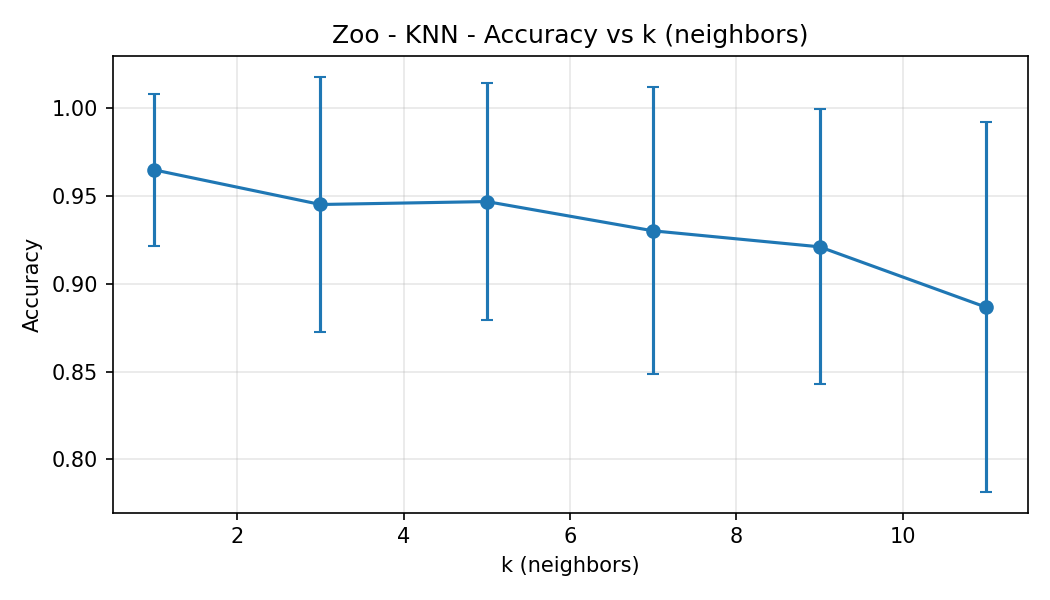
\includegraphics[width=0.9\textwidth]{outputs/extra_credit2_zoo/knn_accuracy.png}
  \caption{Extra Credit \#2 (Zoo): k-NN accuracy plot.}
  \label{fig:zoo-knn}
\end{figure}

\begin{figure}[!htbp]
  \centering
  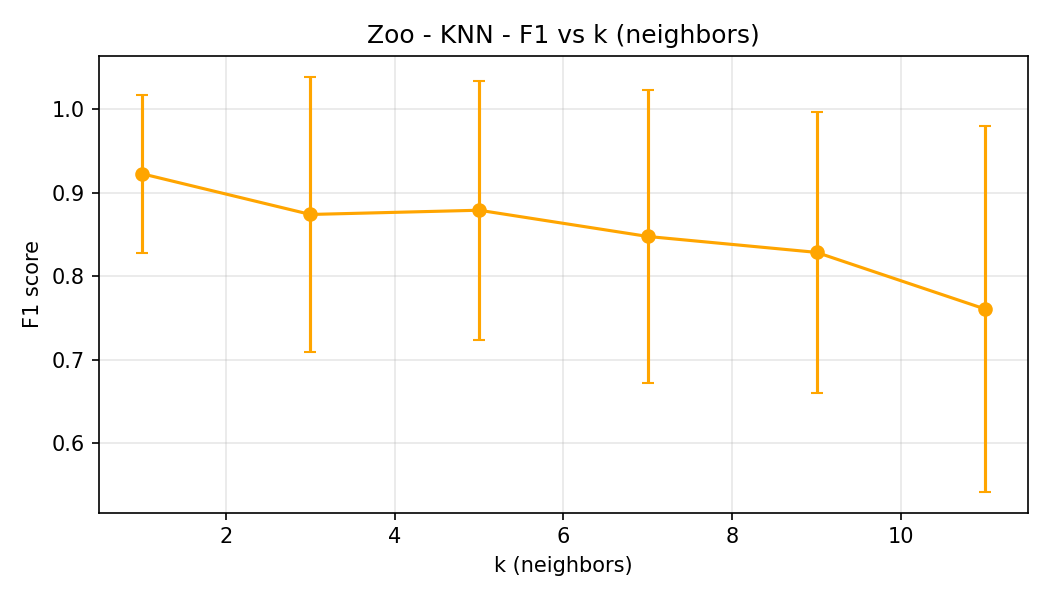
\includegraphics[width=0.9\textwidth]{outputs/extra_credit2_zoo/knn_f1.png}
  \caption{Extra Credit \#2 (Zoo): k-NN F1 plot.}
  \label{fig:zoo-knn-f1}
\end{figure}


\begin{figure}[!htbp]
  \centering
  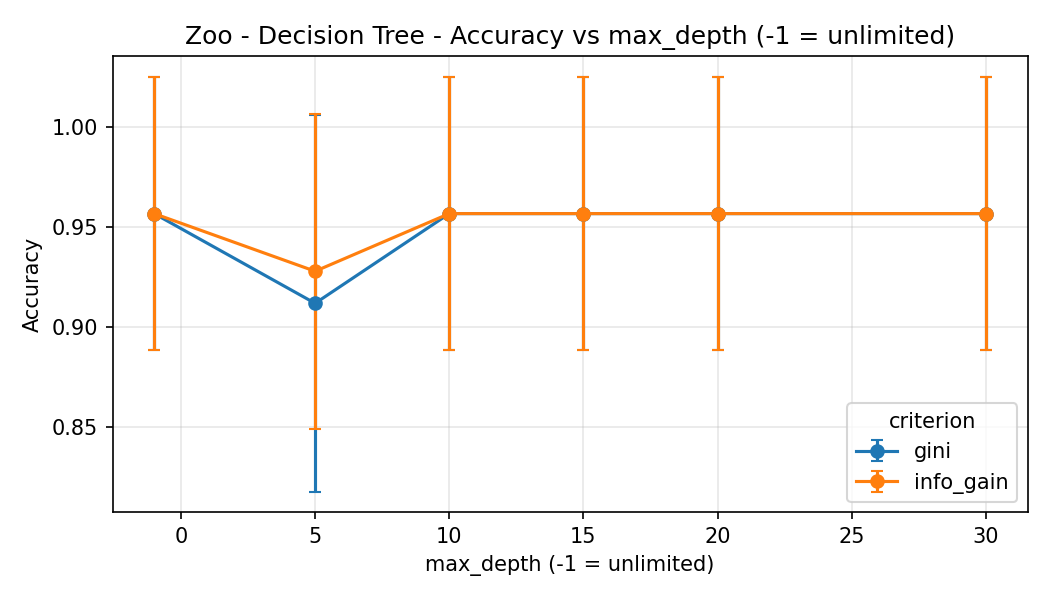
\includegraphics[width=0.9\textwidth]{outputs/extra_credit2_zoo/dt_accuracy.png}
  \caption{Extra Credit \#2 (Zoo): Decision Tree accuracy plot.}
  \label{fig:zoo-dt}
\end{figure}


\begin{figure}[!htbp]
  \centering
  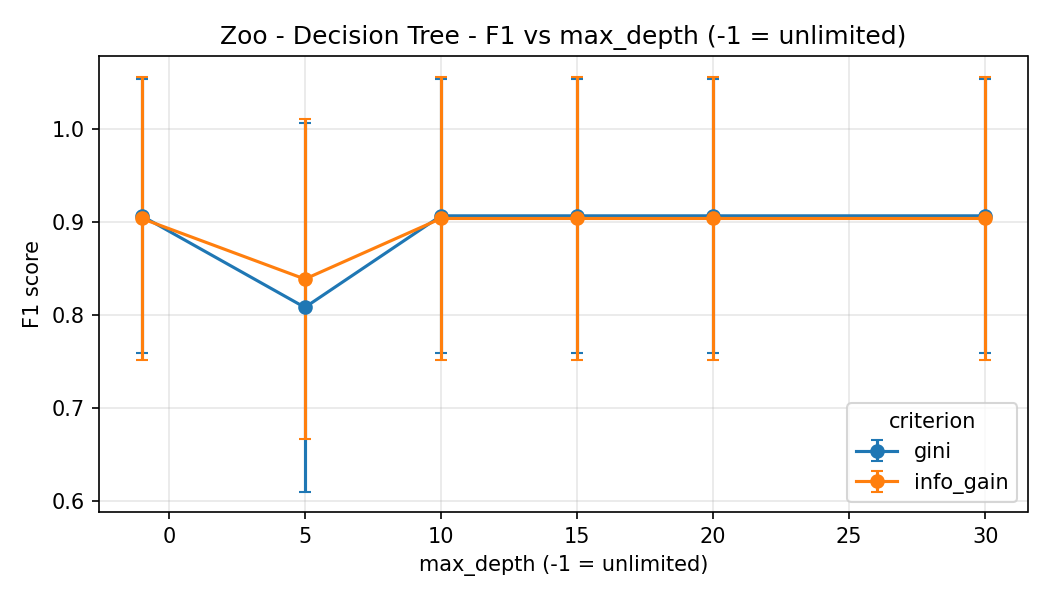
\includegraphics[width=0.9\textwidth]{outputs/extra_credit2_zoo/dt_f1.png}
  \caption{Extra Credit \#2 (Zoo): Decision Tree F1 plot.}
  \label{fig:zoo-dt-f1}
\end{figure}

\begin{figure}[!htbp]
  \centering
  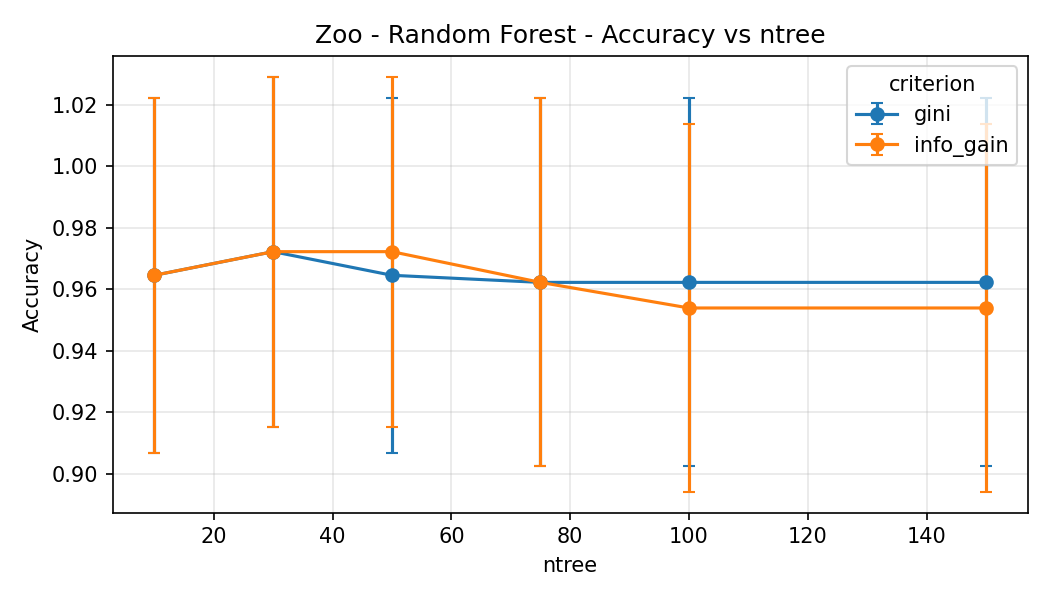
\includegraphics[width=0.9\textwidth]{outputs/extra_credit2_zoo/rf_accuracy.png}
  \caption{Extra Credit \#2 (Zoo): Random Forest accuracy plot.}
  \label{fig:zoo-rf}
\end{figure}

\begin{figure}[!htbp]
  \centering
  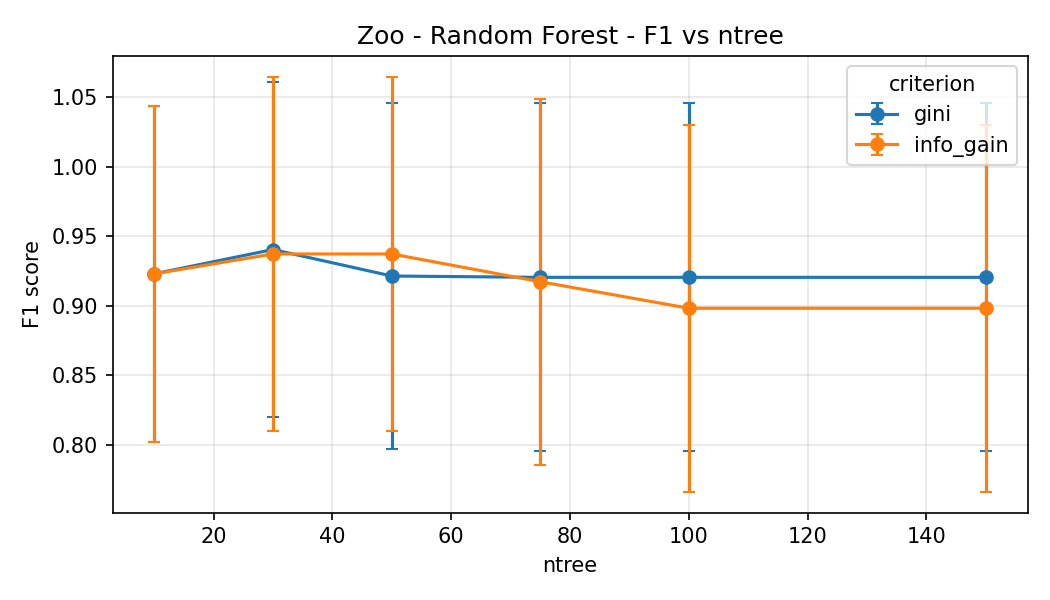
\includegraphics[width=0.9\textwidth]{outputs/extra_credit2_zoo/rf_f1.png}
  \caption{Extra Credit \#2 (Zoo): Random Forest accuracy plot.}
  \label{fig:zoo-rf-f1}
\end{figure}

\begin{figure}[!htbp]
  \centering
  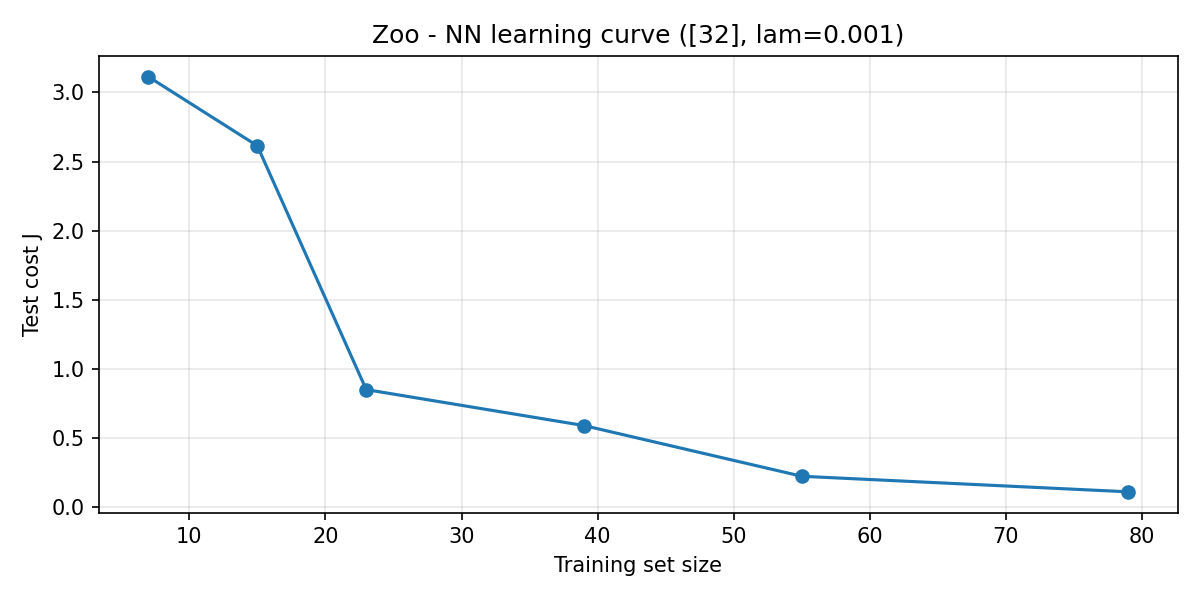
\includegraphics[width=0.9\textwidth]{outputs/extra_credit2_zoo/nn_learning_curve.png}
  \caption{Extra Credit \#2 (Zoo): NN learning curve ($J$).}
  \label{fig:zoo-nn}
\end{figure}

\newpage
\section*{Reproducing results}
\begin{verbatim}
python3 digits.py                       # Run digits dataset
python3 parkinsons.py                   # Run parkinsons dataset
python3 rice.py                         # Run rice dataset
python3 credit.py                       # Run credit dataset
python3 main.py                         # parallel run of all 4 datasets + summaries
python3 extra_credit2.py                # Run Zoo dataset
\end{verbatim}
Raw tables: \\
\filepath{outputs/digits/digits_cv_results.csv}, \\ \filepath{outputs/parkinsons/parkinsons_cv_results.csv}, \\  \filepath{outputs/rice/rice_cv_results.csv},  \\ \filepath{outputs/credit_approval/credit_approval_cv_results.csv}.

\end{document}
